\documentclass[12pt]{article}

%%%%%%%%%%%%%%%%%%%%%%%%%%%%%%%%%%%%%%%%%%%%%%%%%%%%%%%%%%%%%%%%%%%%%%%%%%%%%%%%
% Add packages
%%%%%%%%%%%%%%%%%%%%%%%%%%%%%%%%%%%%%%%%%%%%%%%%%%%%%%%%%%%%%%%%%%%%%%%%%%%%%%%%
\RequirePackage{doi}
\usepackage{latexsym,amsfonts,amssymb,amsthm,amsmath,commath}
\usepackage{indentfirst}
\usepackage[super]{nth}
\usepackage{setspace}
\usepackage{xr-hyper}
\usepackage{hyperref}
\usepackage[capitalise]{cleveref}
\usepackage[utf8]{inputenc}
\usepackage[nottoc,notlot,notlof]{tocbibind}
%\usepackage{background}
\usepackage{graphicx}
\usepackage{chngcntr}
\usepackage{bookmark}
\usepackage{appendix}
\usepackage{siunitx}
\usepackage{physics}
\usepackage{natbib}
\usepackage{xcolor}
\usepackage{xspace}
\usepackage{bbold}
\usepackage{float}
\usepackage{url}
\usepackage{bm}


%%%%%%%%%%%%%%%%%%%%%%%%%%%%%%%%%%%%%%%%%%%%%%%%%%%%%%%%%%%%%%%%%%%%%%%%%%%%%%%%
% Package configurations
%%%%%%%%%%%%%%%%%%%%%%%%%%%%%%%%%%%%%%%%%%%%%%%%%%%%%%%%%%%%%%%%%%%%%%%%%%%%%%%%
\numberwithin{equation}{section}
\providecommand{\units}[1]{\,\ensuremath{\mathrm{#1}}\xspace}
\setlength{\parindent}{20pt}
\setlength{\oddsidemargin}{0in}
\setlength{\textwidth}{6.5in}
\setlength{\textheight}{8.8in}
\setlength{\topmargin}{0in}
\setlength{\headheight}{18pt}

\newcommand{\N}{\mathbb{N}}
\newcommand{\Z}{\mathbb{Z}}
\newcommand{\R}{\mathbb{R}}
\newcommand{\Q}{\mathbb{Q}}
\newcommand{\PP}{\mathbb{P}}
\newcommand{\HH}{\mathcal{H}}
\newcommand{\xhat}{\vb{\hat{x}}}
\newcommand{\yhat}{\vb{\hat{y}}}
\newcommand{\zhat}{\vb{\hat{z}}}

\DeclareMathOperator{\di}{d\!}
\theoremstyle{definition}
\newtheorem{theorem}{Theorem}[section]
\newtheorem{corollary}{Corollary}[theorem]
\newtheorem{lemma}[theorem]{Lemma}
\newcommand*\Eval[3]{\left.#1\right\rvert_{#2}^{#3}}

\doublespacing

\graphicspath{
    {./figures/}
}
\usepackage{lineno}

\begin{document}

%\maketitle
\begin{titlepage}
\vspace*{\stretch{1.0}}
\begin{center}

\Large{\textbf{Utilizing the Hamiltonian dynamics to study resonant interactions
of whistler-mode waves and electrons in the solar wind}} \\
\vspace{2.5cm}
\vspace{2.5cm}
\begin{abstract}
    To study the interaction of solar wind electrons and large-amplitude
    whister waves, a vectorized test particle simulation was developed with a 
    variational component to calculate the Lyapunov exponents. A description of 
    particle dynamics using the Hamiltonian formulation and secular 
    perturbation theory confirmed that the electron's pitch angle diffusion was 
    along the constant Hamiltonian surface and that it was driven by the 
    interaction with the resonance surfaces. Also, the role of large-amplitude
    whistlers in the scattering of solar wind electrons was established. Oblique
    whistlers were shown to be able to efficiently scatter field-aligned strahl
    electrons into the halo population in the solar wind. These waves were 
    capable of generating horn-like features in the velocity distribution 
    function, consistent with the behavior reported in recent PIC studies.
\end{abstract}

\vspace{2.5cm}

\end{center}
\vspace*{\stretch{2.0}}
\end{titlepage}

\newpage

\singlespacing
\tableofcontents
\doublespacing

\newpage
\linenumbers
\section{Introduction}\label{sec:intro}
\begin{figure}[h]
    \centering
    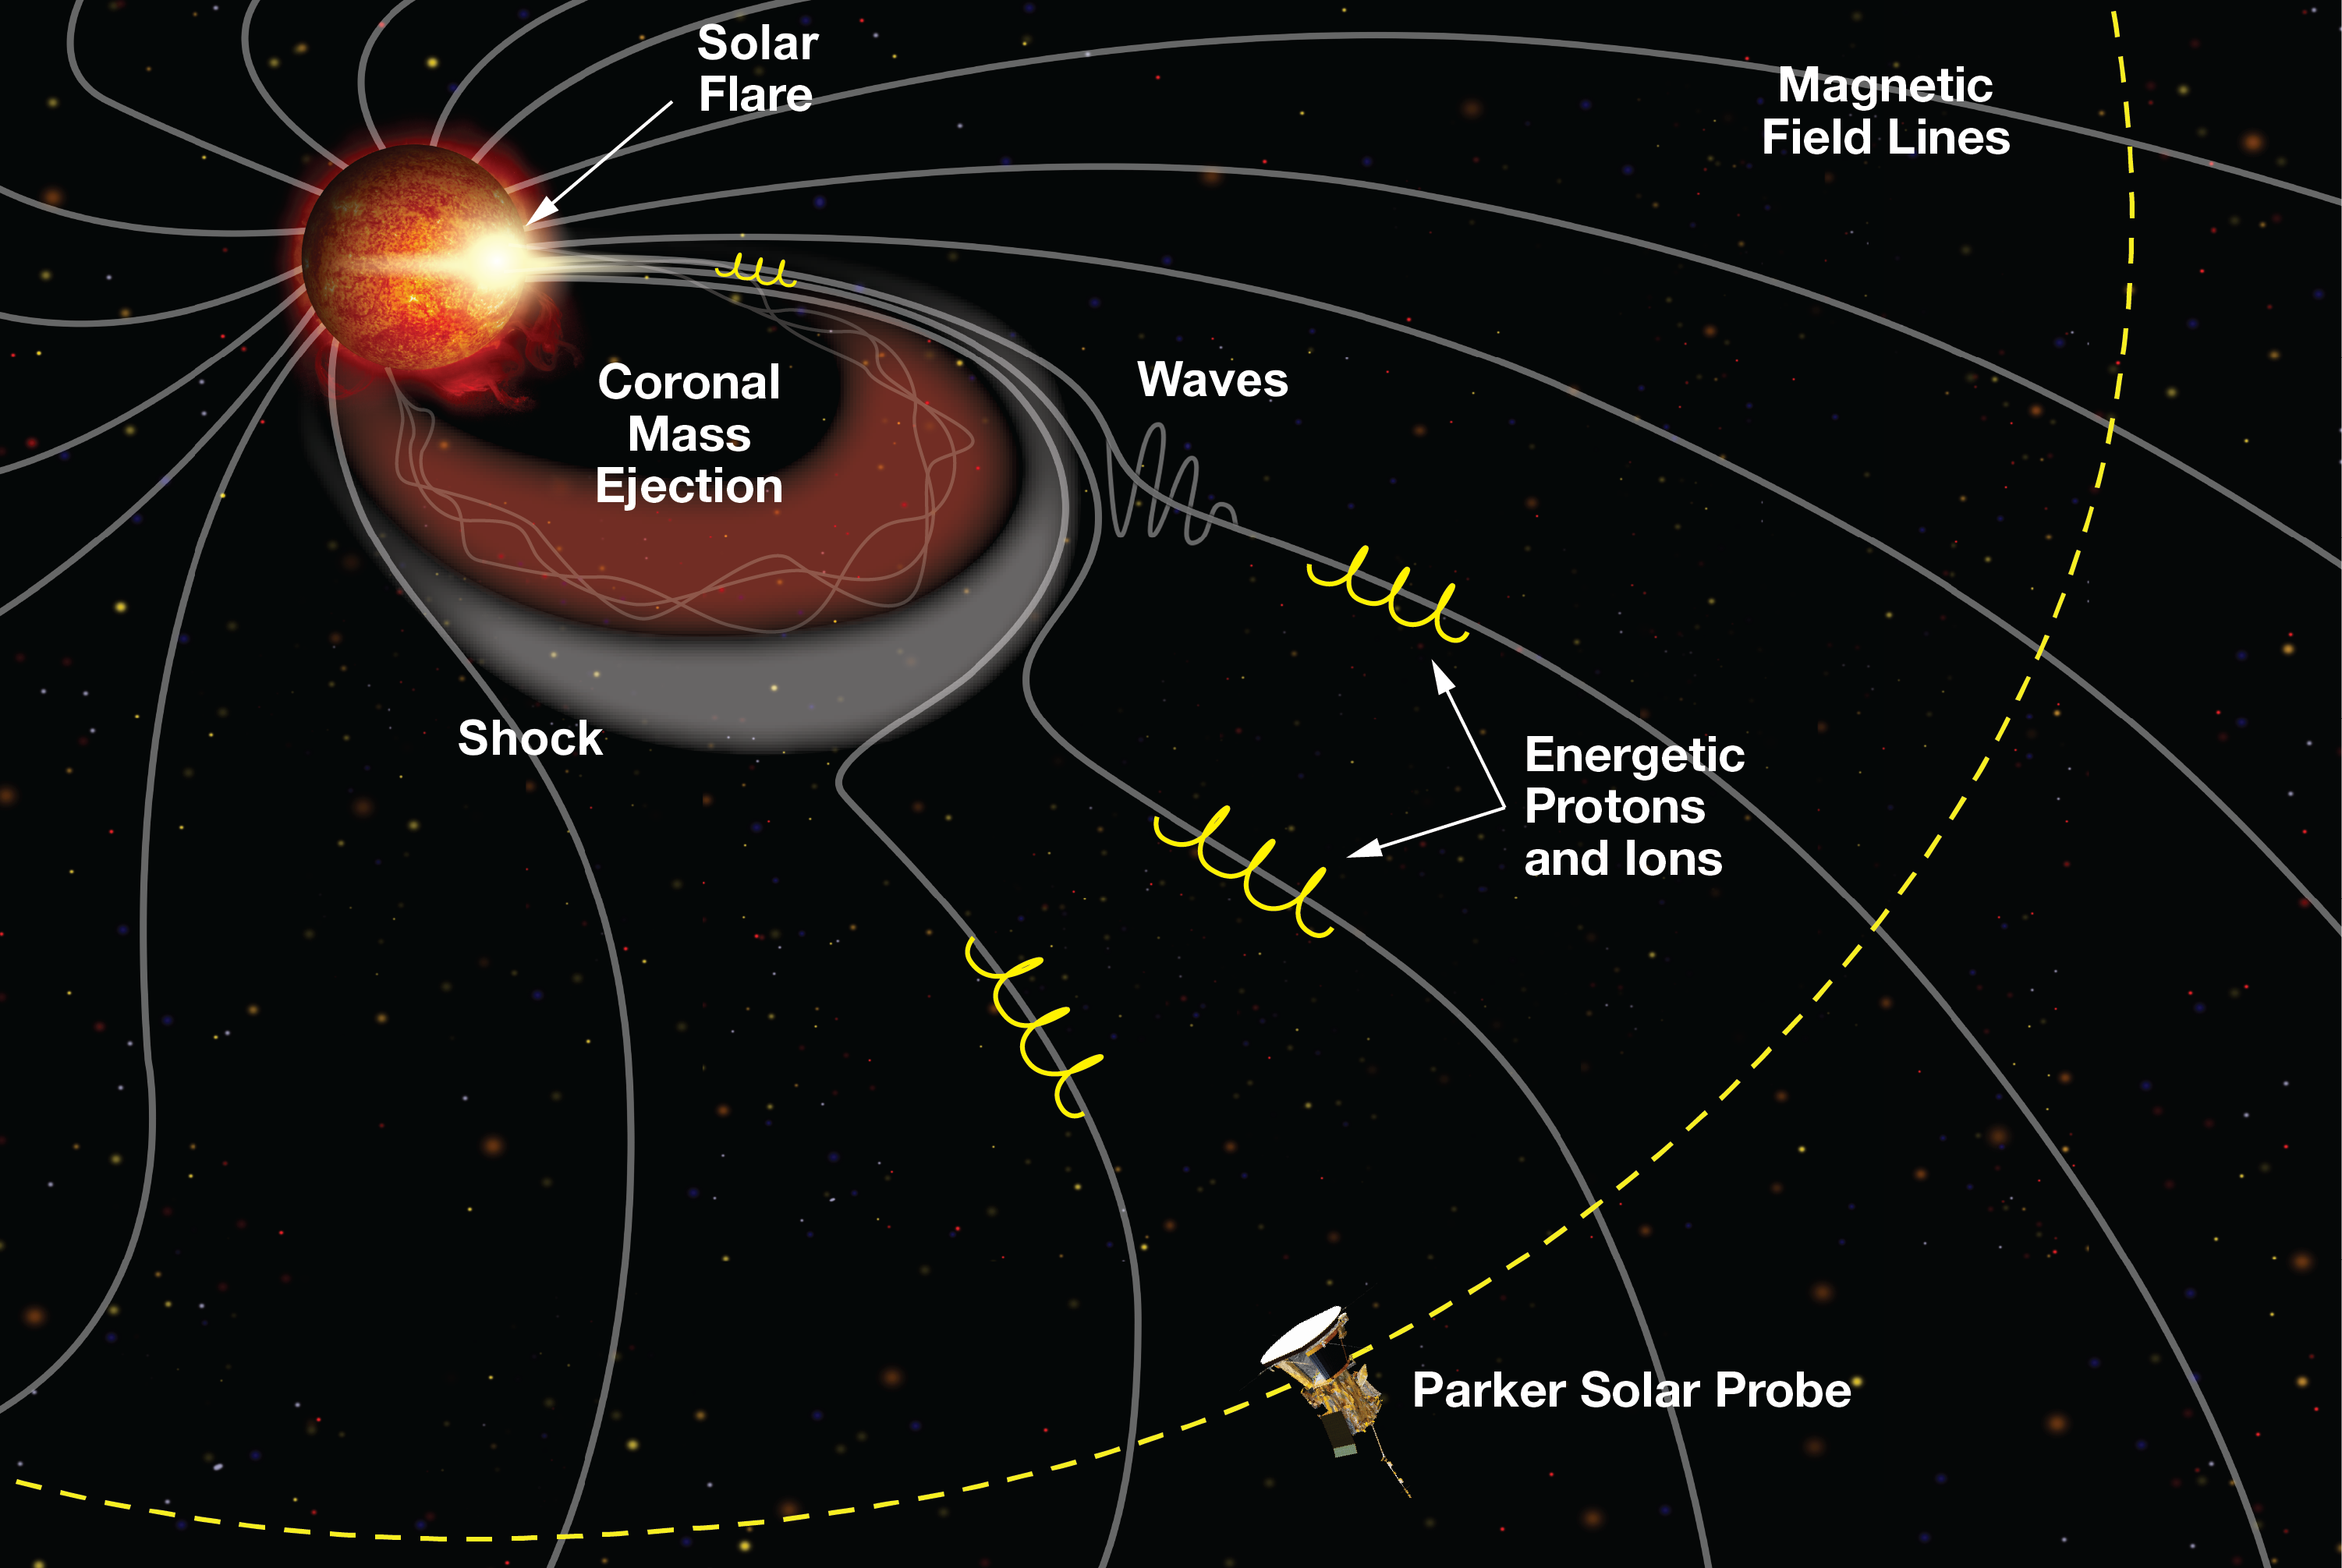
\includegraphics[width=0.7\textwidth]{parker_spirals.png}
    \caption{The spiral geometry of the solar wind and the
    interplanetary magnetic field lines (source: \cite{NASA}).}
    \label{fig:spirals}
\end{figure}

The solar wind originated from the solar corona is a magnetized
and nearly collisionless plasma consisting primarily of electrons, protons, and
alpha particles. Typically, it can be described as a magnetohydrodynamic fluid
with a very high magnetic Reynold's number. Consequently, the magnetic field at
the solar surface is frozen into the solar wind plasma and carried along with
it. This results in a spiraled geometry of the interplanetary magnetic field
lines called the Parker spirals (see \cref{fig:spirals}). \cite{Parker1958}
found from this geometry that the magnetic field followed an inverse square law
$B_r\sim r^{-2}$ and the particle density $n\sim r^{-2}V^{-1}$ also decreased
with increasing speed $V$ and radial distance $r$.

\begin{figure}
    \centering
    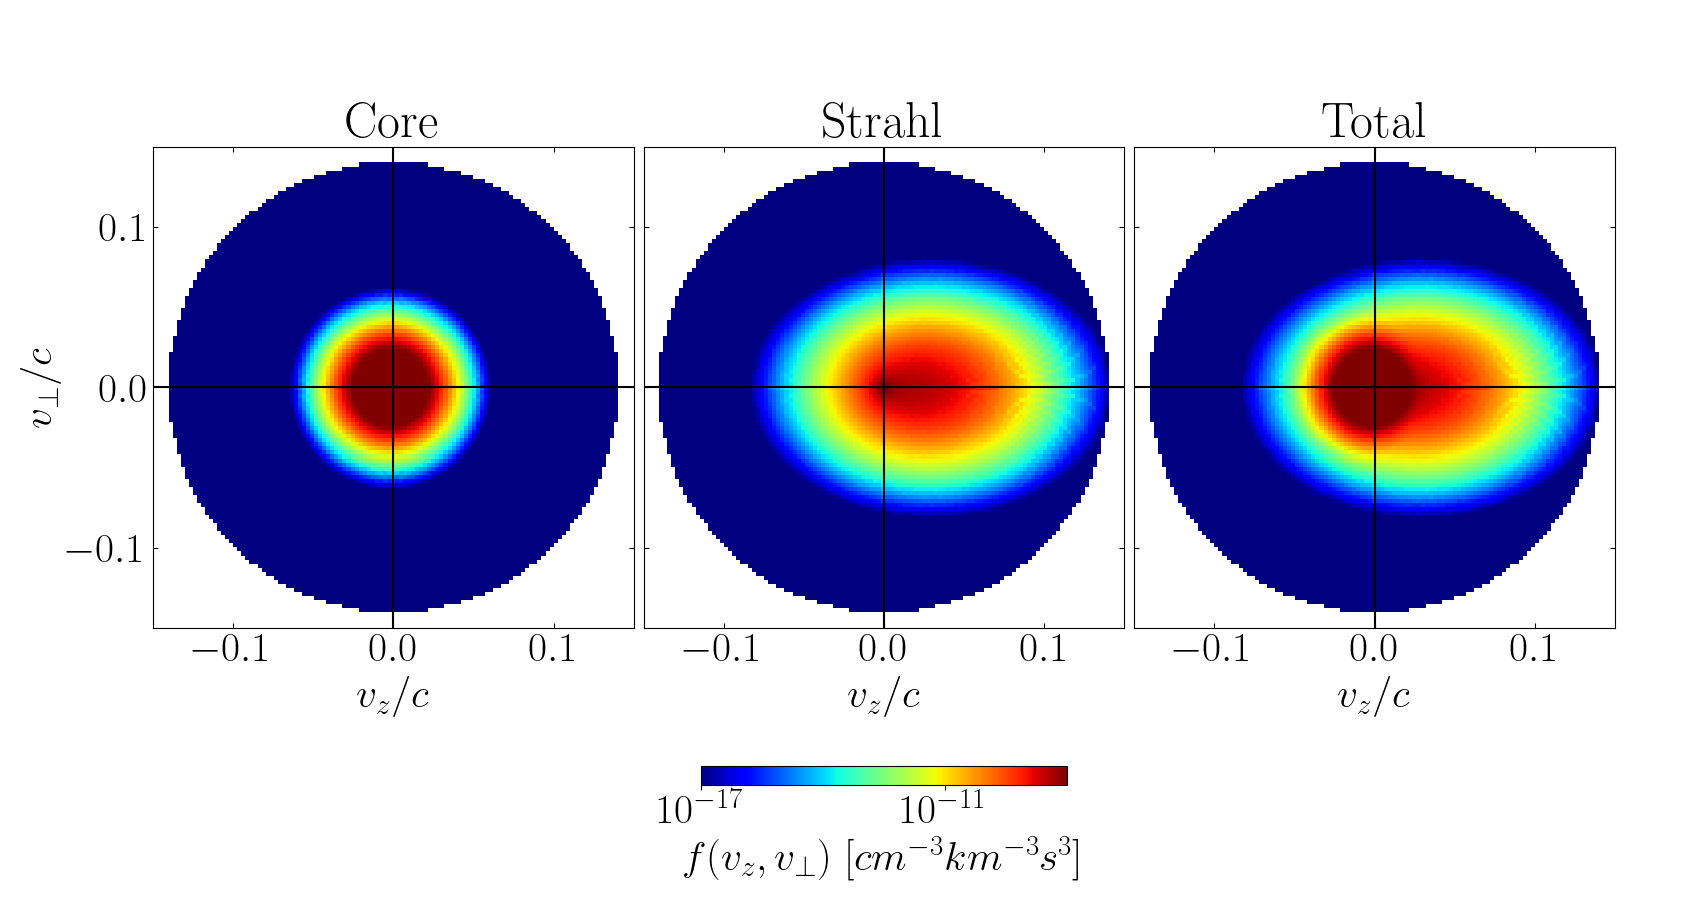
\includegraphics[width=\textwidth]{original_0.3_AU.png}
    \caption{Model of initial electron populations at 0.3 AU used in the
        simulations in \cite{Micera2020}. The core and
    strahl bulk velocity ensures zero net current.}
    \label{fig:03_AU_particles}
\end{figure}

In the velocity distribution of solar wind electrons, observations have shown
that there are usually three populations, a cold core, a hot halo, and a magnetic field aligned strahl, which evolve with heliospheric distance
\citep{Montgomery1968,Feldman1975,Pilipp1987}. Observations near the Sun (0.3 AU) from the Parker Solar Probe (PSP) have reported that the halo almost disappears, while the strahl is narrower than further out from the Sun \citep{Halekas2020}. \cref{fig:03_AU_particles} shows an example of the velocity
distribution function (VDF) of electrons at 0.3 AU, where both core and
strahl populations are modelled with a bi-Maxwellian distribution. Far from the
Sun, statistical studies at 1 AU from \cite{Maksimovic2005} and \cite{Wilson2019} have modelled core electrons with a bi-Maxwellian distribution, while the halo and the strahl are better fitted with a bi-Kappa distribution (see \cref{fig:solar_wind_electrons}).
\begin{figure}
    \centering
    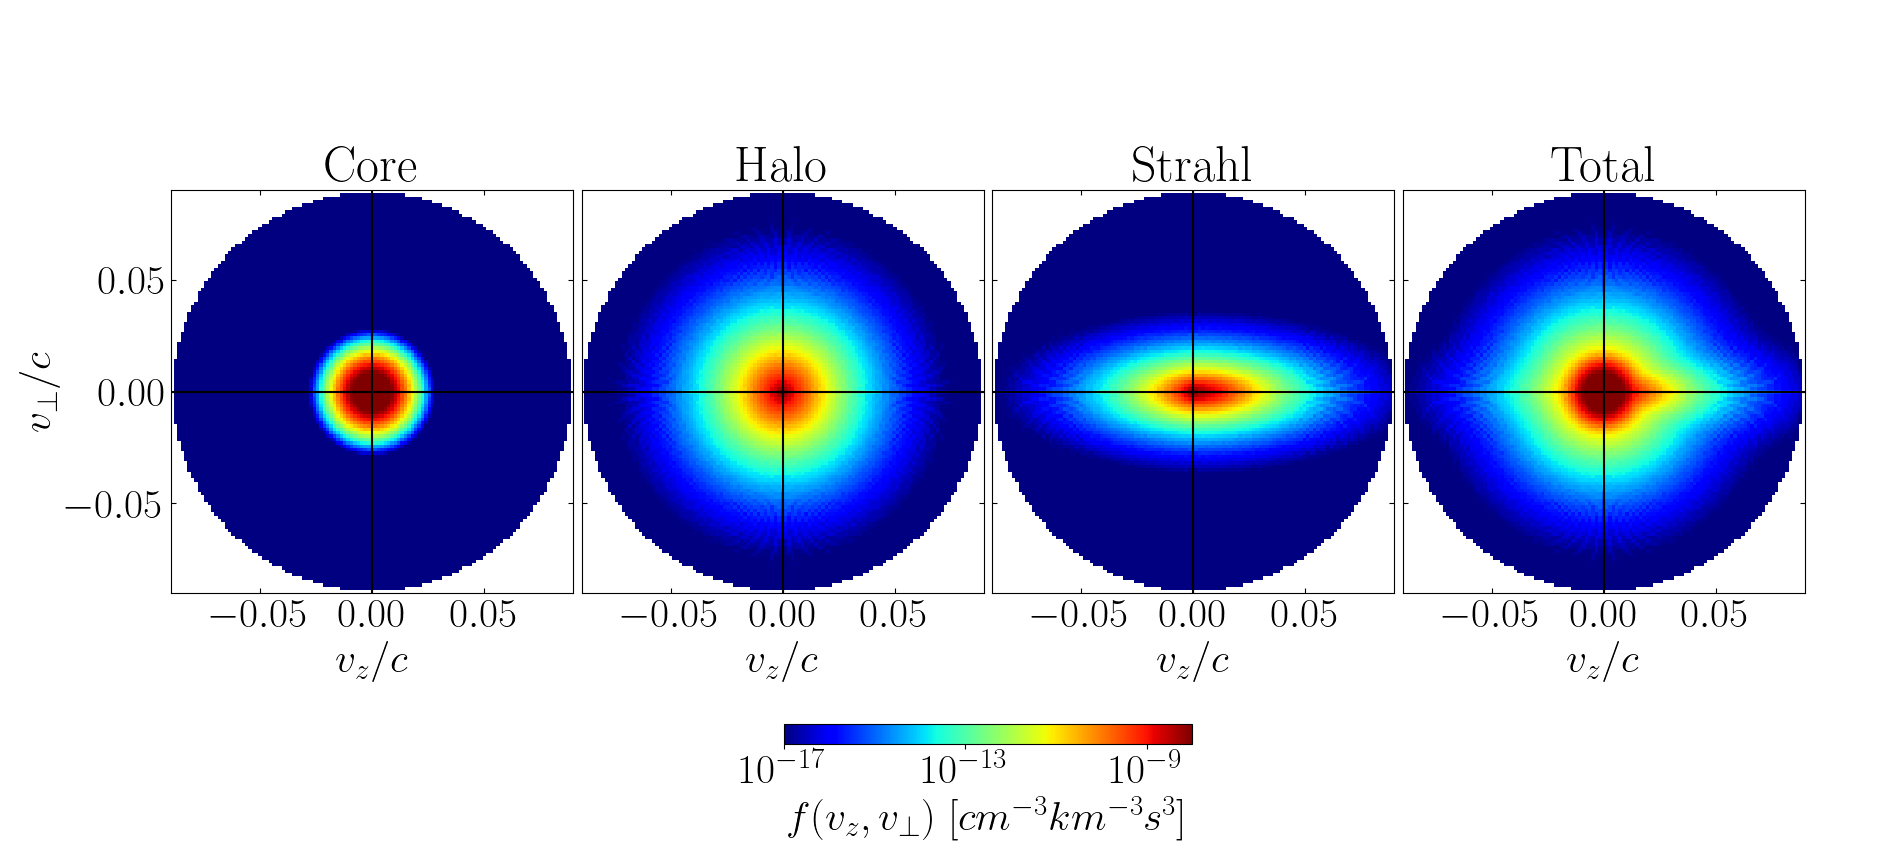
\includegraphics[width=\textwidth]{original_1_AU.png }
    \caption{Components of solar wind electrons
observed by the Wind satellite at 1 AU as fitted by \cite{Wilson2019}.}
    \label{fig:solar_wind_electrons}
\end{figure}

As these electrons stream radially out, if their propagation were adiabatic,
meaning the magnetic moment $\mu\sim v_\perp^2/B_r$ were conserved, then the
perpendicular velocity would have to decrease. This means far from the Sun, the
strahl should be increasingly narrow. However, in-situ data have shown an
opposite trend in the radial evolution of solar wind electrons.
\cite{Stverak2009} observed from 0.3 to 1 AU that the strahl density decreased
as the halo density increased by the same amount relative to the core (see
\cref{fig:density_radial_evolution}). This suggests that the origin of the halo
is due to the scattering of the strahl. Additionally, \cite{Anderson2012} and
\cite{Graham2017} reported that the strahl's pitch angle width distribution
varied greatly from 5 to 90$^\circ$ at 1 AU and increased radially beyond 1 AU.
Thus, it would be harder to identify a field aligned strahl population further
out from the Sun.

\begin{figure}
    \centering
    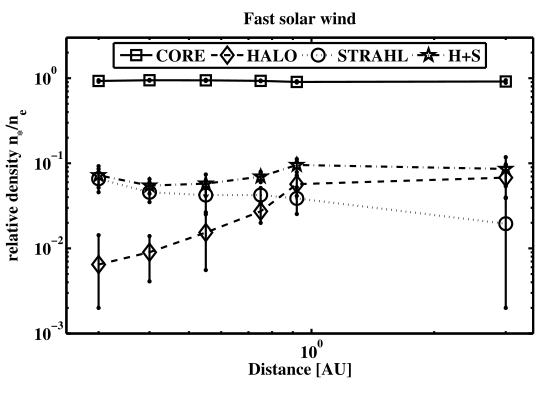
\includegraphics[width=0.48\textwidth]{density_evolution_fast.png}
    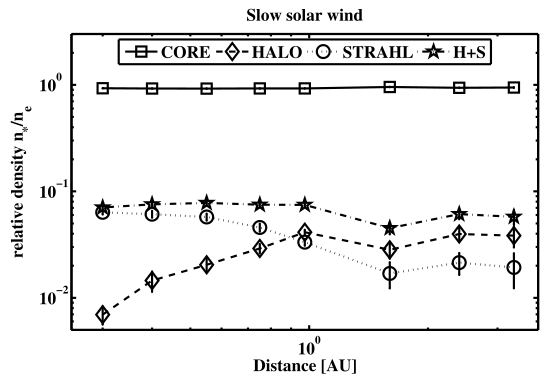
\includegraphics[width=0.497\textwidth]{density_evolution_slow.png}
    \caption{Radial evolution of electrons in the fast and slow
    solar wind from 0.3 to 6 AU \citep{Stverak2009}.}
\label{fig:density_radial_evolution}
\end{figure}

Therefore, there must be a mechanism that scatters strahl
electrons into the halo distribution. Wave-particle interaction is one such
process that allows the energization and scattering of resonant electrons.
Specifically, whistler-mode waves, a right-hand polarized electromagnetic wave,
have long been proposed as a candidate to explain these solar wind observations.
Through theoretical and simulation studies, they have been demonstrated to
scatter electrons in the Earth's radiation belts \citep[][and references
therein]{Karimabadi1990,Albert1993,Tao&Bortnik2010,Hsieh2017}. However,
these studies typically focused on small whistler amplitudes with $\delta
B/B_0\sim\mathcal{O}(10^{-4})$. \cite{Breneman2010} and \cite{Cattell2020} used
electric field waveform captures from the STEREO satellites at 1 AU and
demonstrated that large amplitude, narrowband, obliquely propagating whistlers
were frequently present in the solar wind. They were observed in the range of
$5$--$40$\,\si{mV/m}, which corresponds to $\delta B/B_0\sim\mathcal{O}(0.1)$.
These large amplitude whistlers recently became an interest because of
new data from the PSP at 0.3 AU. \cite{Agapitov2020} and \cite{Cattell2021} 
observed large amplitude waves of this order near the Sun. Additionally, their
polarization indicated that the propagation varied from quasi-parallel to
oblique angles. \cite{Micera2020} simulated whistlers from heat-flux
instabilities near the Sun using electron distributions modeled after PSP
data and showed the halo formation from strahl electrons. \cite{RobergClark2019} reported the formation of ``horns'' in
velocity space due to the scattering of resonant strahl electrons with oblique
whistlers in solar flares (see \cref{fig:vdf_horns}). Thus, we are interested in
studying the scattering and energization of solar wind electrons due to these
large amplitude waves and comparing our results with observations and these recent simulations.

\begin{figure}
    \centering
    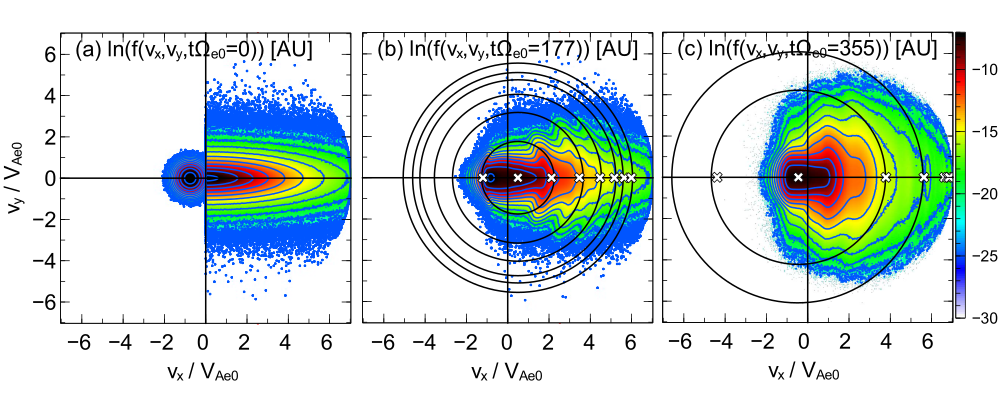
\includegraphics[width=\textwidth]{vdf_horns.png }
    \caption{Formation of horns in velocity space of an
        original distribution (a) of core and strahl
        electrons \citep{RobergClark2019}. The horizontal and vertical axes are
    the parallel and perpendicular velocity normalized by the electron Alfvén
    speed. Panel (b) shows the resulting interaction with a right-ward wave.
The white crosses are the $n=-5,-4,...,1$ resonances. Panel (c) shows that with
a left-ward wave (with $n=-1,0,...,5$ resonances).}
    \label{fig:vdf_horns}
\end{figure}


%\begin{figure}
%    \centering
%    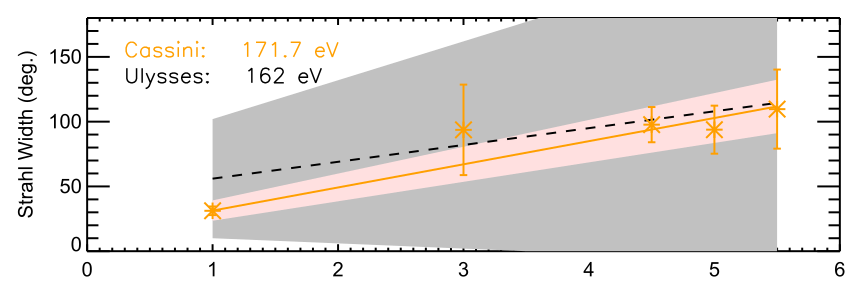
\includegraphics[width=\textwidth]{strahl_width.png }
%    \caption{Radial evolution of the strahl's pitch angle width beyond 1AU \citep{Graham2017}.}
%    \label{fig:strahl_width}
%\end{figure}

\cite{Kersten2014} developed a test particle
simulation to study whistler-electron interactions in the radiation belts
and later adapted it to simulate whistlers at stream interaction regions in the
solar wind based on observations in \cite{Breneman2010}. Modelled after the
simulation in \cite{Roth1999}, the code used a fourth order Runge-Kutta (RK)
integration algorithm to solve the Lorentz equation numerically. This is a
general approach to numerical problems as the RK family of integrators is known
to produce highly precise solutions. The results are therefore reliable as long as one is interested in single-particle behaviors. However, this approach fails to maintain the consistency among a spectrum of initial conditions as the solutions might be more unstable for certain regions in phase space. For the high amplitude waves of interest, chaotic behavior is usually present. Thus, this program is insufficient to investigate the behavior of an electron distribution as it provides no physical measure to judge the reliability among the results.

Particle-In-Cell (PIC) simulations, as used by \cite{Micera2020} and
\cite{RobergClark2019}, are a standard in plasma research in studying
self-consistently evolving systems. Instead of a high order RK algorithm, they
usually use a time-centered, second-order explicit integrator called the Boris
pusher \citep{Birdsall&Langdon1985}. Although not a symplectic algorithm,
it is the \textit{de facto} method for advancing a charged particle in an
electromagnetic field because the Boris pusher conserves local phase space
volume \citep{Qin2013}. This means the energy error is globally bounded for an
arbitrarily large number of time steps. Thus, this numerical method is capable
of resolving multi-scale dynamical problems over a long simulation period.
However, PIC simulations are computationally expensive, as they solve Maxwell
equations along with advancing particles and usually handle millions to
trillions of particles. For our purpose, large scale PIC simulations are not
necessary, because test particle simulations allow us to examine the interaction
for different wave properties and over all particle angles and energies.


In this thesis, a vectorized test particle simulation capable of
investigating the behavior of a distribution of hundreds of thousands of
electrons is utilized. The code is modelled after the Vector Particle-In-Cell 
(VPIC) code using only the particle advancing component \citep{Bowers2008}. In
\cref{sec:theory}, a derivation of the whistler wave fields from a cold, 
collisionless plasma dispersion relation is given. Also, the Hamiltonian
analysis of the resonance surface using Hamilton-Jacobi and perturbation theory
is discussed. In \cref{sec:simulation}, detail of the calculations in the
simulation are laid out, together with the estimation of the Lyapunov exponents 
to measure the efficiency of the integration algorithm.
\cref{sec:diagnostics} presents the diagnostics of the simulation including the 
Lyapunov exponents, the adiabatic invariants, and whistler parameters. 
\cref{sec:analysis} reports simulation results of the electron distribution 
interactions with single uniform whistlers and a narrowband packet of whistlers 
at 0.3 AU and 1 AU and their analysis as according to quasi-linear
resonant theory. Conclusions and suggestions for future works are in
\cref{sec:conclusion,sec:future_works}.


\section{Theory}\label{sec:theory}
\subsection{Equations of whistler wave fields}\label{sec:whistler}

In a cold uniform plasma with a background magnetic field
$\vb{B}_0=B_0\zhat$, the electric
permittivity tensor is
\begin{equation}
    \bm\epsilon=\epsilon_0\bm\epsilon_R=\epsilon_0\mqty(S&-iD&0\\iD&S&0\\0&0&P)
\end{equation}
where the constants $S,D,P$ are the Stix parameters \citep{Stix1992} given as
follows
\begin{equation}
    S=1-\sum_s\frac{\omega_{ps}^2}{\omega^2-\Omega_{cs}^2}, \qquad
    D=\sum_s\frac{\abs{q_s}}{q_s}\frac{\Omega_{cs}\omega_{ps}^2}{\omega\qty(\omega^2-\Omega_{cs}^2)},
    \qquad P=1-\sum_s\frac{\omega_{ps}^2}{\omega^2}
\end{equation}
The summation is over all species $s$ with charge $q_s$, mass $m_s$, and density
$n_s$.  The plasma frequency is $\omega_{ps}=\sqrt{n_sq_s^2/\epsilon_0m_s}$, and
$\Omega_{cs}=\abs{q_s}B_0/m_s$ is the cyclotron frequency. Now, let there be an
electromagnetic wave propagating in the $(xz)$ plane with
$\vb{k}=k_\bot\xhat+k_\parallel\zhat=k\qty(\sin\theta\xhat+\cos\theta\zhat)$.
Assume also that the fields are Fourier transformed so that $\grad\to i\vb{k}$
and $\partial/\partial t\to-i\omega$. From Maxwell equations, the electric
field satisfies
$\vb{N}\times\qty(\vb{N}\times\vb{E})+\bm\epsilon_R\vdot\vb{E}=0$ where
$\vb{N}=c\vb{k}/\omega$ is the refractive index.  This can be written in the
form $\vb{R}\vdot\vb{E}=0$ where $\vb{R}$ satisfies
\begin{equation}
    \det\vb{R}=\det\mqty(
        S-N_\parallel^2 & -iD & N_\bot N_\parallel\\
        iD & S-N^2 & 0\\
        N_\bot N_\parallel & 0 & P-N_\bot^2
    )=0
\end{equation}
from which the refractive index can be solved. Plugging it back into
$\vb{R}\vdot\vb{E}=0$ yields the electric field polarizations. The right-hand
polarized solution with frequencies between $\Omega_{ci}$ and $\Omega_{ce}$ is called the whistler mode whose fields can be written in
the form
\begin{subequations}\label{eq:whistler_EM_fields}
 \begin{align}
    \vb{B}_w&=B_x^w\sin\psi\xhat + B_y^w\cos\psi\yhat + B_z^w
    \sin\psi\zhat\label{eq:whistler_magnetic_field}\\
    \vb{E}_w&=E_x^w\cos\psi\xhat-E_y^w\sin\psi\yhat+E_z^w\cos\psi\zhat\label{eq:whistler_electric_field}
\end{align}
\end{subequations}
where the wave phase is $\psi=\vb{k}\vdot\vb{r}-\omega t$ and the magnetic field
is given by Faraday's law $\vb{B}_w=(1/\omega)\vb{k}\times\vb{E}_w$. The
polarizations are summarized in \cite{Tao&Bortnik2010}
\begin{align}\label{eq:whistler_polarizations}
    E_x^w/E_x^w&=1 &
    E_y^w/E_x^w&=\frac{D}{N^2-S} &
    E_z^w/E_x^w&=-\frac{N^2\sin\theta\cos\theta}{P-N^2\sin^2\theta}\notag\\
    cB_x^w/E_x^w&=\frac{ND\cos\theta}{N^2-S} &
    cB_y^w/E_x^w&=\frac{NP\cos\theta}{P-N^2\sin^2\theta} &
    cB_z^w/E_x^w&=\frac{ND\sin\theta}{S-N^2}
\end{align}

For the analysis of the Hamiltonian, it is also necessary to find a scalar and
vector potential representing the above fields. Assuming the general form for
the whistler potentials used in \cite{Karimabadi1990} and \cite{Roth1999}, we
can find the amplitudes such that they are consistent with
\cref{eq:whistler_EM_fields}.  Suppose the scalar potential is
$\Phi_w=\Phi_0\sin\psi$ and the vector potential is
\begin{equation}\label{eq:vector_potential}
    \vb{A}_w=A_1\qty(\frac{k_\parallel}{k})\sin\psi\xhat+A_2\cos\psi\yhat-A_1\qty(\frac{k_\bot}{k})\sin\psi\zhat
\end{equation}
Equating the corresponding electric field
$\vb{E}=-\grad\Phi_w-\partial\vb{A}_w/\partial t$ to
\cref{eq:whistler_electric_field}, we can solve for $\Phi_0,A_1$, and $A_2$ as
follows.
\begin{align}
    \Phi_0&=-\frac1{k}\qty[\qty(\frac{k_\bot}{k})E_x^w+\qty(\frac{k_\parallel}{k})E_z^w]
          &
    A_1&=\frac1\omega\qty[\qty(\frac{k_\parallel}{k})E_x^w-\qty(\frac{k_\bot}{k})E_z^w]
       &
    A_2&=\frac{E_y^w}{\omega}
\end{align}


\subsection{Particle dynamics}\label{sec:particle_dynamics}

The curvature of the Parker spiral is small over a length scale of
$\sim100\,000\,$\si{km}, which we will later confirmed through comparison with
the particle motion. We can therefore assume the background field is uniform
$\vb{B}_0=B_0\zhat$. Given a vector potential $\vb{A}=\vb{A}_w+xB_0\yhat$ and a scalar potential $\Phi_w$ where $\vb{A}_w,\Phi_w$ are defined as in \cref{sec:whistler}, the relativistic Hamiltonian for a particle with mass $m$ and charge $q$, is
 \begin{equation}\label{eq:relativistic_hamiltonian}
    \HH=\sqrt{m^2c^4+\qty(\vb{P}-q\vb{A}_w-qB_0x\yhat)^2c^2}+q\Phi_w
 \end{equation}
 where $\vb{P}=\gamma m\vb{v}+q\vb{A}$ is the canonical momentum conjugate to
 the Cartesian coordinates and $\gamma$ is the Lorentz factor.

 There are two issues. First, note that $\HH$ depends on $x$, so
 $\dot{P_x}=-\partial\HH/\partial x\neq0$ and $P_x$ is not invariant. Secondly,
 $\vb{A}_w$ oscillates with the phase $\psi(x,z,t)$. So the energy is not
 conserved as the Hamiltonian is time-dependent. The former is a standard
 problem since $\HH$ is currently formulated in Cartesian coordinates, whereas
 the system is cylindrically symmetric due to the background magnetic field.
 This can be resolved by transforming into a cylindrical frame
 \citep{Goldstein2002}. The latter is, however, more problematic as the wave
 introduces oscillations symmetric about its direction of propagation. In-depth
 analysis of the Hamiltonian can be done by using secular perturbation theory
 \citep{Lichtenberg&Lieberman1992}, which involves decomposing the Hamiltonian into Bessel-Fourier series and performing the gyro-averaging method to separate a single term, the $n$th harmonic, in the series.


 Within the scope of our analysis, we will calculate this Hamiltonian system's
 adiabatic invariants and derive its resonance surfaces similar to
 the approach of \cite{Karimabadi1990} and \cite{RobergClark2019}.  The mathematical details are given in \cref{sec:hamiltonian_analysis}. For motion near the resonance $n$, the Hamiltonian can be recast into the form
 \begin{equation}\label{eq:1D_hamiltonian}
     \HH(\zeta;\hat{P_\phi},\hat{P_\zeta})
     =\gamma\qty(\hat{P_\phi}+n\hat{P_\zeta},k_\|\hat{P_\zeta})mc^2
     -\omega\hat{P_\zeta}
     +G_n\qty(\hat{P_\phi}+n\hat{P_\zeta},k_\|\hat{P_\zeta})\sin\zeta
 \end{equation}
 where the action-angle variables $(\zeta,\hat{P_\zeta})$ and $(\phi,\hat{P_\phi})$ are
 given by
 \begin{align}
     \zeta&=n\phi+k_\bot P_y/qB_0+k_\| z-\omega t &
     \phi&=\tan^{-1}\qty[\frac{m\Omega_c\qty(x-P_y/qB_0)}{P_x}]\notag\\
     \hat{P_\zeta}&=P_\|/k_\| & \hat{P_\phi}&=P_\phi-nP_\|/k_\|=P_\perp^2/2m\Omega_c-nP_\|/k_\|
 \end{align}
 The perpendicular momentum is defined as
 $P_\perp=\sqrt{P_x^2+\qty(P_y-qB_0x)^2}$. The gyroradius is then
 $\rho=P_\perp/m\Omega_c=\sqrt{2P_\phi}$, and
 the Lorentz factor $\gamma=\sqrt{1+(P_\perp^2/m^2c^2)+(P_\|^2/m^2c^2)}$.
 The perturbation amplitude $G_n$ is defined as
 \begin{equation}
     G_n(P_\phi,P_\|)=mc^2\qty{s\qty[\delta_0+\frac{\delta_1}{\gamma}\qty(\frac{k_\perp}{k}\frac{P_\|}{mc}-\frac{k_\|}{k}\frac{n\Omega_c}{ck_\perp})]J_n\qty(k_\bot\sqrt{2P_\phi})+\frac{\delta_2}{\gamma}\frac{\rho\Omega_c}{c}J_n'\qty(k_\perp\sqrt{2P_\phi})}
 \end{equation}
 where $J_n,J_n'$ are the $n$th order Bessel functions of the first kind and
 their derivatives, the wave potential amplitudes are
 $\delta_0=\abs{q}\Phi_0/mc^2$ and $\delta_{1,2}=\abs{q}A_{1,2}/mc$, and
 $s=q/\abs{q}$ is the charge sign. The equation of motion of this system is
 \begin{subequations}\label{eq:hamiltonian_eom}
    \begin{align}
        \frac{d\zeta}{dt}&=-\omega+\frac{n\Omega_c}{\gamma}+\frac{k_\|P_\|}{\gamma m}+\qty(n\frac{\partial
        G_n}{\partial P_\phi}+k_\|\frac{\partial G_n}{\partial
    P_\|})\sin\zeta\label{eq:dzdt}\\
            \frac{d\hat{P_\zeta}}{dt}&=-G_n\cos\zeta\label{eq:dPdt}
    \end{align}
 \end{subequations}

 \begin{figure}
     \centering
     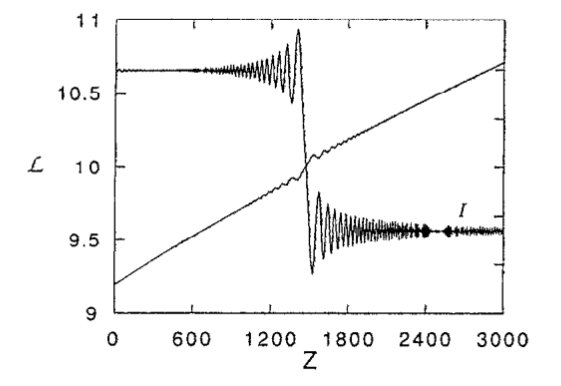
\includegraphics[width=0.6\textwidth]{resonance_crossing.png}
     \caption{The change in the adiabatic invariant $I$ as the resonance
     $\mathcal{L}$ crosses an integer value (figure from \cite{Albert1993}).
 In our notations, $\mathcal{L}=n$, $I=\hat{P_{\phi}}$, and $Z=z$.}
     \label{fig:resonance_crossing}
 \end{figure}
 Here, we have assumed that the wave is small ($\delta_{0,1,2}\ll
 1$ and $\delta_{1,2}<\gamma v/c$, where $v$ is the particle's velocity). So the
 motion $\dot\zeta$ is usually fast, meaning we can average over $\zeta$
 and $\dot{P_\zeta}=0$, except for when
 \begin{equation}\label{eq:resonant_condition}
     \omega=\frac{n\Omega_c}{\gamma}+\frac{k_\|P_\|}{\gamma m}
 \end{equation}
 The adiabatic invariant $\hat{P_\zeta}$ is no longer conserved whenever the particle undergoes a resonance crossing (see \cref{fig:resonance_crossing}). \cref{eq:resonant_condition} then
 describes a resonant condition. Although this is not a convention, most
 literature defines the gyrophase as $s\phi$, which results
 in the resonant mode being $sn$. For an electron with $s=-1$, this means
 their fundamental cyclotron motion is the $n=-1$ mode, while the fundamental
 cyclotron as defined by \cref{eq:resonant_condition} is $n=1$. This definition 
 will be used in subsequent discussions. 

\begin{figure}
     \centering
     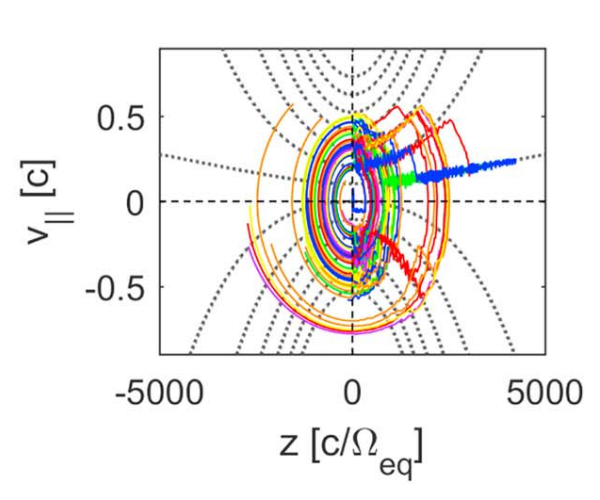
\includegraphics[width=0.6\textwidth]{hsieh_particle_trapped.png}
     \caption{Trajectories (colored solid lines) of particles being trapped
         along (dotted) resonance lines
     ($\abs{n}\leq6$) in \cite{Hsieh2017}.}
     \label{fig:trapped_particles}
 \end{figure}

\subsection{Resonance surfaces}\label{sec:resonance_surfaces}


Using the dynamics we established in \cref{sec:particle_dynamics},
we can use a tool provided by \cite{Karimabadi1990}, the resonance-diagram
technique. The derivation steps are included in
\cref{sec:RH_surface_derivation}. Let $H_0=\gamma-v_p(P_\|/mc)$ be the
normalized unperturbed Hamiltonian in \cref{eq:1D_hamiltonian} where
$v_p=1/N_\|=\omega/k_\|c$ is the normalized phase velocity and $N_\|$ the
parallel refractive index. A constant value of $H_0$ defines a constant energy
($H$) surface in phase space $(P_\|,P_\bot)$. In the non-relativistic limit,
this is the equation of a circle centered around $v_p$ with $(v_\|/c-v_p)^2+v_\perp^2/c^2=\text{const}$ \citep{RobergClark2019}. In the relativistic limit, the $H$ surface is elliptic
\begin{equation}\label{eq:constant_H_surface}
    \frac{(v_\|-v_c)^2/c^2}{R_0/(H_0^2+v_p^2)}+\frac{v_\perp^2/c^2}{R_0/H_0^2}=1
\end{equation}
where $v_c/c=v_p/(H_0^2+v_p^2)$ and $R_0=H_0^2-1+v_p^2/(H_0^2+v_p^2)$. We have approximated $P\approx \gamma
mv$ (which is valid if the particle term dominates in the canonical momentum)
and write the surface in terms of the observable $v$. Similarly, one can also
define a resonance ($R$) surface from the resonant condition
\cref{eq:resonant_condition}. Its intersections to the $v_\perp=0$ axis
are
\begin{equation}\label{eq:resonant_velocity}
    v_{r,\|}=\frac{v_p}{1+\alpha_n^2}\pm\sqrt{\frac{\alpha_n^2}{1+\alpha_n^2}\qty(1-\frac{v_p^2}{1+\alpha_n^2})}
\end{equation}
where $\alpha_n=n\Omega_c/k_\|c$. The Landau resonance $(n=0)$ is located at the
center of all $H$ surfaces and other pairs of resonance
($n=\pm1,\pm2,\pm3,\hdots$) are equidistant to that center (see
\cref{fig:vdf_horns} for examples from the Roberg-Clark simulation). For whistler waves, $N_\|$ is usually larger than 1, so the maximum energization is highly limited because the number of $H$--$R$ intersections are small \citep{Karimabadi1990}. Thus, particles tend to move along the constant $H$ surface until they interact resonantly with the wave near the $H$--$R$ intersection and become energized or de-energized. In subsequent sections,
only particles in the non-relativistic energy range where $H$ is circular and
$R$ is approximately a constant surface at $v_z=v_{r,\|}$ will be investigated. 
In subsequent analysis, the particles' trajectories in phase space will be
confirmed to follow this behavior.



\section{Simulation}\label{sec:simulation}
\subsection{Particle advance}
The Hamiltonian equation of motion in \cref{eq:hamiltonian_eom}, although useful
for analysis, is only an approximation near a single resonance. \cite{Roth1999}
alternated between that and the exact Lorentz force to reduce the computational cost for particles entering resonance, since adaptive RK of the 4th order is
expensive. However, in doing so, the code user must impose an arbitrary boundary
in switching between the resonant and non-resonant regimes. Here, we shall use
the relativistic Boris pusher from \cite{Ripperda2018} to solve for the full
Lorentz force and rely on its volume-preserving characteristics to choose the
appropriate step size. However, we must first describe our normalizations. From
\cref{sec:whistler}, it is natural to normalize $\vb{B}\to\vb{B}/B_0$ and
subsequently $\vb{E}\to \vb{E}/cB_0$. Since we are using relativistic
formulations, $\vb{v}\to\vb{v}/c$ and $\vb{P}\to\vb{P}/mc$. The characteristic
frequency in our system is defined by the electron cyclotron frequency
$\Omega_{ce}$, so the wave frequency $\omega\to\omega/\Omega_{ce}$ and time
$t\to t\Omega_{ce}$. The spatial position thus becomes $\vb{r}\to\vb{r}\Omega_{ce}/c$.

The description of the Boris algorithm is as follows. The Lorentz force in
natural units has the form $d\vb{u}/dt=s\qty(\vb{E}+\vb{v}\times\vb{B})$ where
$\vb{u}=\gamma\vb{v}$ and $\gamma=\sqrt{1+u^2}$. The time-centered finite difference expression of this is
\begin{equation}
 \vb{u}_{n+1}-\vb{u}_n=s\Delta
t\qty[\vb{E}_n+\qty(1/2\gamma_n)\qty(\vb{u}_{n+1}+\vb{u}_n)\times\vb{B}_n]
\end{equation}
 where $\vb{u}_n=\gamma_n\vb{v}\qty(t_n-\Delta t/2)$, $\vb{E}_n=\vb{E}_n(t_n)$,
$\vb{B}_n=\vb{B}_n\qty(t_n)$ and $\Delta t$ is the step size where
$t_n=n\Delta t$ for $n\in\N$. $\gamma_n$ is the Lorentz factor determined from
$u_n$. Now, the Kick-Drift-Kick steps that make this algorithm a leapfrog scheme
are defined via the two auxilliary vectors $\vb{u}_\pm$. The first kick is a
half electric field acceleration from $\vb{u}_n$ to $\vb{u}_-=\vb{u}_n+(s\Delta
t/2)\vb{E}_n$, followed by a rotation $\vb{u}_-\to\vb{u}_+$ by the magnetic
field $\vb{u}_+=\vb{u}_-+\qty(\Delta
t/2\gamma_n)(\vb{u}_++\vb{u}_-)\times\vb{B}_n$. $\vb{u}_+$ here seems to be
implicitly defined, but from the geometry of this rotation, it can be computed
explicity as $\vb{u}_+=\vb{u}_-+\qty(\vb{u}_-+\vb{u}_-\times\vb{T})\times\vb{S}$
with $\vb{T}=\qty(s\Delta t/2\gamma_n)\vb{B}_n$ and $\vb{S}=2\vb{T}/(1+T^2)$
(see more details in \cite{Birdsall&Langdon1985}). Then the second kick accelerates the particle to the next state $\vb{u}_{n+1}=\vb{u}_++\qty(s\Delta
t/2)\vb{E}_n$.

To simulate a single uniform whistler fields in natural units,
\cref{eq:whistler_EM_fields} can be rewritten as
\begin{equation}\label{eq:simulate_B}
    \frac{\vb{B}_w}{B_0}=\frac{E_x^w}{cB_0}\qty[\qty(\frac{cB_x^w}{E_x^w})\sin\psi\xhat+\qty(\frac{cB_y^w}{E_x^w})\cos\psi\yhat+\qty(\frac{cB_z^w}{E_x^w})\sin\psi\zhat]
\end{equation}
and similarly,
\begin{equation}\label{eq:simulate_E}
    \frac{\vb{E}_w}{cB_0}=\frac{E_x^w}{cB_0}\qty[\cos\psi\xhat-\qty(\frac{E_y^w}{E_x^w})\sin\psi\yhat+\qty(\frac{E_z^w}{E_x^w})\cos\psi\zhat]
\end{equation}
Since the STEREO spacecraft only measured the whistler electric field amplitudes
\citep{Breneman2010}, $E_x^w$ is used as
the scaling factor. The unitless polarizations can be computed with
\cref{eq:whistler_polarizations}. Note that the wave phase in natural units
is $\psi=\omega\qty(N_\perp x+N_\|z-t)$, and that it is zero for particles
starting out at the origin at $t=0$. Originally, the wave has an amplitude
$E_{w}^0=E_x^w\sqrt{1+\qty(E_z^w/E_x^w)^2}$. So, $E_x^w$ will be chosen such
that $E_{w}^0$ has a desired physical value. To simulate a wave packet with
the same original wave amplitude $E_{w}^0$ and $N$ frequencies
$\omega_j=\omega_1+(j-1)\Delta\omega$ with spacing $\Delta\omega$, the
calculations \cref{eq:simulate_B} and \cref{eq:simulate_E} can simply be
repeated and the total fields are $\vb{E}_w=\sum_{j=1}^N\vb{E}_{w,j}$ and
$\vb{B}_w=\sum_{j=1}^N\vb{B}_{w,j}$.

With these calculations, a description of the particle advance at each time step
is completed. The scaling factor is calculated at the beginning of the
simulation. So each loop involves (a) calculating new wave phase, constructing
the total field, and advancing the particle, (b) the diagnostics, and (c)
writing to database. (b) and (c) can be activated at different time intervals.



\subsection{Estimation of the Lyapunov exponents}\label{sec:sim_LCE}


As mentioned in the previous section, the Boris pusher guarantees a
volume-preserving characteristic. To verify that our simulation's step size is
sufficiently small that the algorithm efficiently preserves volume in phase
space, we employ a concept from chaos theory called the Lyapunov exponents
\citep{Ott2002}. These exponents essentially describe how a basis spanning a $k$-dimensional space changes under subsequent transformations. For simplicity, suppose we have a 1-D trajectory. If the Lyapunov exponent is $\lambda=0$, then the space (distance, in this case) around it evolves as $\exp\qty(n\lambda)=1$
and doesn't contract or expand after $n$ time steps. If $\lambda<0$, the space
eventually reduces to a singular point. This is called an attractor where all
trajectories starting out near this one being considered converges. If
$\lambda>0$, all trajectories originally close together eventually diverge and
become increasingly far from each other. In higher dimensions, these distortions
can be described through the basis elements that span the phase space (see
\cref{fig:ball_expansion}).

\begin{figure}
    \centering
    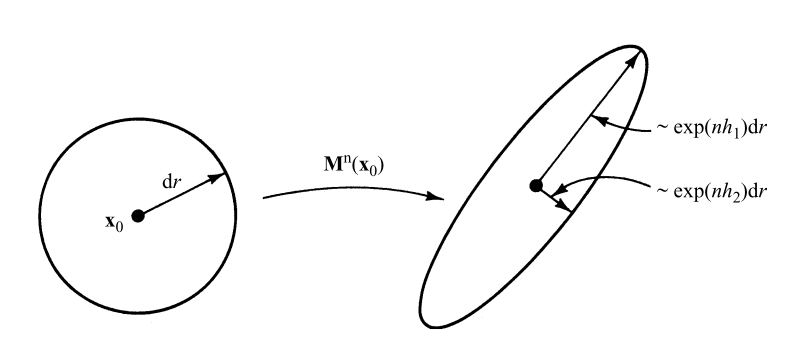
\includegraphics[width=0.8\textwidth]{ball_expansion.png}
    \caption{Distortion of a two-dimensional ball after $n$ time steps.
    $h_1,h_2$ are the Lyapunov exponents in each axial direction spanning the
ball.}
    \label{fig:ball_expansion}
\end{figure}

It requires infinitely many vectors near a point in phase space to compute the
Lyapunov exponents precisely. Thus, one can only estimate the values using a
variety of methods. Here, we shall use a variational approach with Gram-Schmidt
orthogonalization \citep{Benettin1980,Sandri1996}. Given an initial condition to
our ordinary differential equations (ODEs) in the previous section, we can
attach to it a six-dimensional ``ball'' given by a
6x6 matrix, or a set of six 6-D column vectors $U_0=\qty{\vb{u}_j}_{j=1}^6$. This choice of a 6-ball is arbitrary, but the
6-D identity map $\mathbb{1}_6$ is an obvious option. It becomes
$U_1=\vb{M}_0\vdot{U_0}$ after a local expansion $\vb{M}_0=\mathbb{1}_6+\Delta
t\grad\vb{F}_0$ where $\Delta t$ is the step size and $\grad\vb{F}_0$ is the
Jacobian of our ODEs at $n=0$. More details about $\vb{M}$ and $\grad\vb{F}$ can be found in
\cref{sec:expansion_operator}. By the Gram-Schmidt procedure, we can find a
6-D orthogonal basis $W_1=\qty{\vb{w}_j}_{j=1}^6$ from $U_1$. The volume of the
parallelpiped spanned by this new basis is
$V_1(W_1)=\prod_{j=1}^6\norm{\vb{w}_j}$. Now, the definition of the largest
Lyapunov exponent (LCE) after time $t$ is $\lambda=\lim_{t\to\infty}(1/t)\ln
V$ where $V$ is the current volume of the 6-ball. So after $N$ time steps, the
LCE can be approximated as
\begin{equation}
    \lambda=\frac1{N\Delta t}\sum_{n=1}^N\sum_{j=1}^6\ln\norm{\vb{w}_j^n}
\end{equation}
where $t\to N\Delta t$ and $\vb{w}_j^n$ are the basis elements $j$ at time step
$n$. Note the volume is accumulative through time. It is also possible to define separately the Lyapunov exponent in each dimension of the original 6-ball
\begin{equation}
    \lambda_j=\frac1{N\Delta t}\sum_{n=1}^N\ln\norm{\vb{w}_j^n}
\end{equation}
Then the LCE is just the sum of $\lambda_j$ over 6 dimensions. Our calculations
thus involve consecutively computing at each step $n$ the volume of the ball
from $W_n$ and then renormalizing it to measure the expansion of the next
advance. The final result is an accumulation of the volume expansion through $N$
time steps, from which the LCE can be calculated.



\section{Diagnostics}\label{sec:diagnostics}


\subsection{Wave parameters}

\begin{figure}[t]
    \centering
    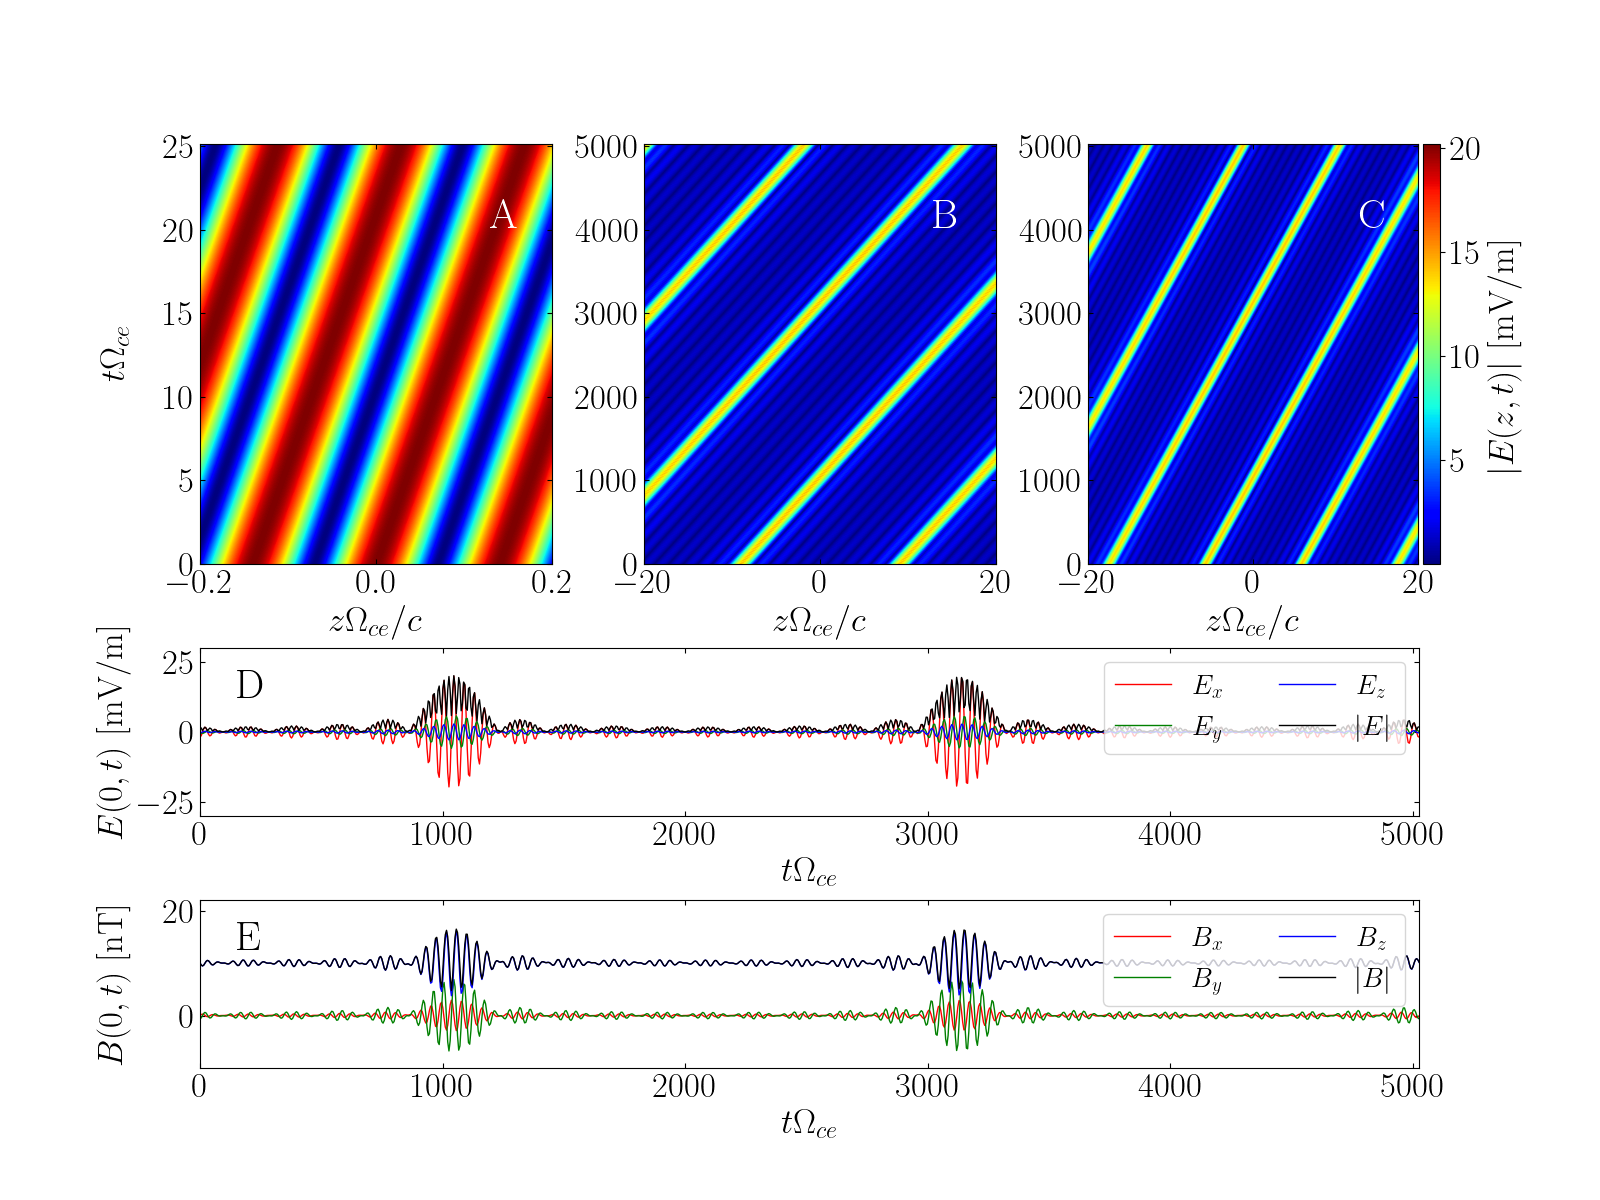
\includegraphics[width=\textwidth]{combo.png}
    \caption{The spatiotemporal evolution at $x=y=0$ of the electric field of an
        oblique ($\theta=65^\circ$) single whistler (A) and oblique whistler
    packets (B \& C). Panels A and B have background parameters for 1 AU and
panel C is for 0.3 AU. Panels D and E show the electric and magnetic field
components at $z=0$ of the packet in panel B.}
    \label{fig:wavefronts}
\end{figure}

In subsequent sections, the interactions of whistlers with electrons in two sets
of background parameters will be studied. The first one is typical of 1 AU with a background field strength $B_0=10$\,\si{nT}. The plasma is quasineutral with $n=n_i=n_e=5$\,\si{cm\tothe{-3}}. The second is consistent with the simulation at 0.3 AU in \cite{Micera2020} with $B_0=50$\,\si{nT} and
$n=n_i=n_e=300$\,\si{cm\tothe{-3}}. The whistler parameters are based on those of \cite{Cattell2020}. For both sets
of background parameters, the single waves have an amplitude
$E_w^0=20$\,\si{mV/m}, frequency $\omega/\Omega_{ce}=0.15$, and propagation
angles $\theta=$ 5, 65$^\circ$, and 175$^\circ$. Whistler packets will contain a
set of eleven $20$\,\si{mV/m} single whistlers with frequency from 0.135 to
0.165 $\Omega_{ce}$ and propagation angles $\theta=0$, $65^\circ$, and
$180^\circ$.

A few examples showing the oblique wavefronts are shown in panels
A, B, and C of \cref{fig:wavefronts}. The phase velocities are different between 0.3 and 1 AU because the background parameters are different. Panels D and E show in more detail the oblique packet in panel B as observed at the origin in time. In \cite{Cattell2020}, the mean observed amplitude was $\si10$\,\si{mV/m}, while those as high as 40\,\si{mV/m} were also observed. Thus, in this study, we use $20$\,\si{mV/m} which has $\delta B_w/B_0\sim0.6$ to clearly see the possible role of the waves. These large amplitude oscillations can result in highly chaotic behavior in the particle motion. Also, note that we are greatly overestimating the parallel wave amplitudes at 1 AU for the sake of comparison. In reality, parallel whistlers at 1 AU are only observed with $\delta B_w/B_0\sim\mathcal{O}(0.01)$.

\begin{figure}
    \centering
    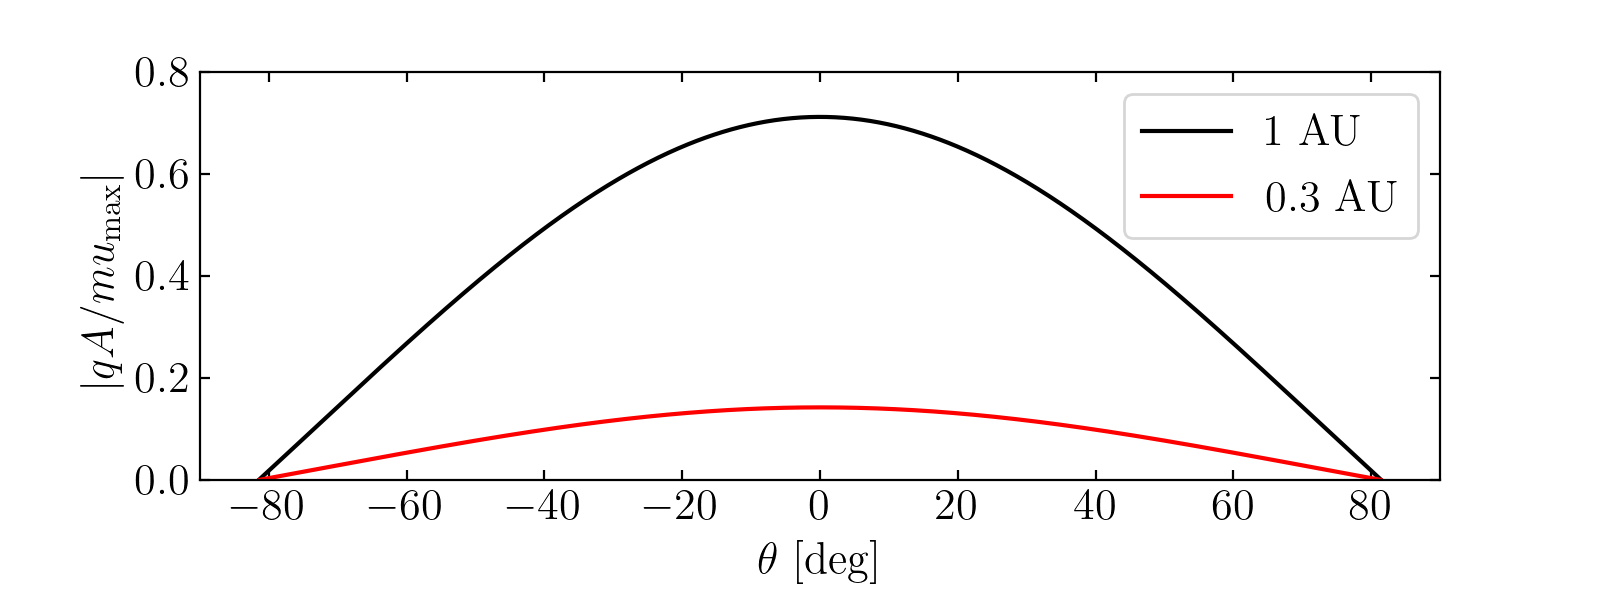
\includegraphics[width=0.95\textwidth]{potential_dominance.png}
    \caption{The ratio between the potential field term $qA$ and the
        particle's relativistic speed term $mu=\gamma mv$ in the canonical
    momentum. $u_{\max}$ corresponds to the maximum kinetic energy of the
simulated electrons. Note that whistlers do not propagate beyond the resonance
cone angle, which is close to 81$^\circ$ but not identical between the black and red
curves \citep{Remya2016}.}
    \label{fig:potential_dominance}
\end{figure}

Since the thermal velocity of electrons in the solar wind is
$\sim2\,000-5\,000$\,\si{km/s}, they are fairly non-relativistic (see
\cref{fig:solar_wind_electrons}). Based on observations of the energy range
for solar wind electrons, particles up to
$\sim$1\,\si{keV} are initiated in the simulations. \cref{fig:potential_dominance} verifies
the small field assumption $\delta_{1,2}<\gamma v/c$ in
\cref{sec:particle_dynamics} for the resonant condition, with $u_{\max}$
corresponding to 1\,\si{keV}. Consequently, $\delta_{1,2}\sim\mathcal{O}(0.01)$
are small compared to unity. So our assumptions regarding the Hamiltonian
derivations are justified, even in the perturbation of these large amplitude
whistlers. For this energy range, the maximum $z$ in our simulations is $\sim30\,000$\,\si{km}, which justifies the assumption of uniform background magnetic field.


\subsection{Particle parameters}

%In a PIC simulation, a weight is attached to each initiated particle, called
%a macroparticle. Each of them resembles a small distribution of electrons and
%together, their motion simulates the evolution of a system of a very large
%number of particles. These macroparticles also have alternated charge, which
%affects the calculation of the charge distribution and consequently the
%electromagnetic field at each time step. However, since we deliberately
%disregard the particles' interaction with the wave and focus on the effect of
%the latter onto the particles instead, we can set their charge to that of an
%electron as is usually done in a test particle simulation. But we will assign a
%weighting function to an adequately large macroparticle distribution to study
%the evolution of electron populations in the solar wind.


As mentioned in \cref{sec:intro}, the two standard velocity distribution
functions (VDF) used to model solar wind electrons are the bi-Maxwellian and the bi-Kappa. The former is
\begin{equation}\label{eq:maxwellian}
    f_M(v_\perp,v_\|)=\frac{n_0}{\pi^{3/2}v_{th,\perp}^2v_{th,\|}}\exp\qty{\qty[\qty(\frac{v_\|-v_{o,\|}}{v_{th,\|}})^2+\qty(\frac{v_\perp-v_{o,\perp}}{v_{th,\perp}})^2]}
\end{equation}
where $v_\|=v_z,v_\perp=\sqrt{v_x^2+v_y^2}$, $v_{th,j}$ is the thermal speed, $v_{o,j}$ is the drift speed in each direction, and $n_0$ is the population density. The bi-Kappa VDF is given by
\begin{equation}\label{eq:kappa}
    f_K(v_\perp,v_\|)=A_\kappa\qty{1+\qty(\kappa-\frac32)^{-1}\qty[\qty(\frac{v_\|-v_{o,\|}}{v_{th,\|}})^2+\qty(\frac{v_\perp-v_{o,\perp}}{v_{th,\perp}})^2]}^{-\qty(\kappa+1)}
\end{equation}
where
$A_\kappa=n_0\pi^{-3/2}\qty(\kappa-3/2)^{-3/2}v_{th,\perp}^2v_{th,\|}\Gamma(\kappa+1)\qty[\Gamma(\kappa-1/2)]^{-1}$. For 1 AU parameters, the core is best modelled by a bi-Maxwellian, while the halo and strahl are best modelled by a bi-Kappa as shown in \cref{fig:solar_wind_electrons} where the maximum kinetic energy is 1\,\si{keV}. The following values are from the mean observations in \cite{Wilson2019}. The initial isotropic core has density
$n_c=13.7$\,\si{cm\tothe{-3}}, zero drift, and
$v_{th}=v_{th,\|}=v_{th,\perp}=1\,800$\,\si{km/s}. The halo is also isotropic
with $n_h=0.52$\,\si{cm\tothe{-3}} and $v_{th}=3\,900$\,\si{km/s}. The strahl
has $n_s=0.21$\,\si{cm\tothe{-3}}, $v_{o,\|}=2\,000$\,\si{km/s}, and
$v_{th,\|}=3v_{th,\perp}=3\,600$\,\si{km/s} (note that it is anisotropic with
$v_{th,\|}\neq v_{th,\perp}$). These VDFs are sampled with
$\sim400\,000$ electrons initiated uniformly in speed with pitch angles (the
polar angle) from 0 to 180$^\circ$ in increments of 1$^\circ$ and gyrophases
(the azimuthal angle) from 0 to 360$^\circ$ in increments of 30$^\circ$. For 0.3
AU, the core and strahl are modelled with the bi-Maxwellian
in parameters similar to \cite{Micera2020}, based on observations by
\cite{Halekas2020} (see \cref{fig:03_AU_particles}). The core has $n_c=332.5$\,\si{cm\tothe{-3}} and $v_{th}=3\,900$\,\si{km/s} with a drift $v_{o,\|}=-480$\,\si{km/s}, while the strahl has $n_s=17.5$\,\si{cm\tothe{-3}}, $v_{th,\|}=7\,900$\,\si{km/s},
$v_{th,\perp}=5\,600$\,\si{km/s}, and $v_{o,\|}=9\,300$\,\si{km/s}.
Approximately a million particles up to 2\,\si{keV} are initiated with the same 
spacing in the solid angle.




\subsection{Single particle responses and LCE estimation}

\begin{figure}[hbtp]
    \centering
    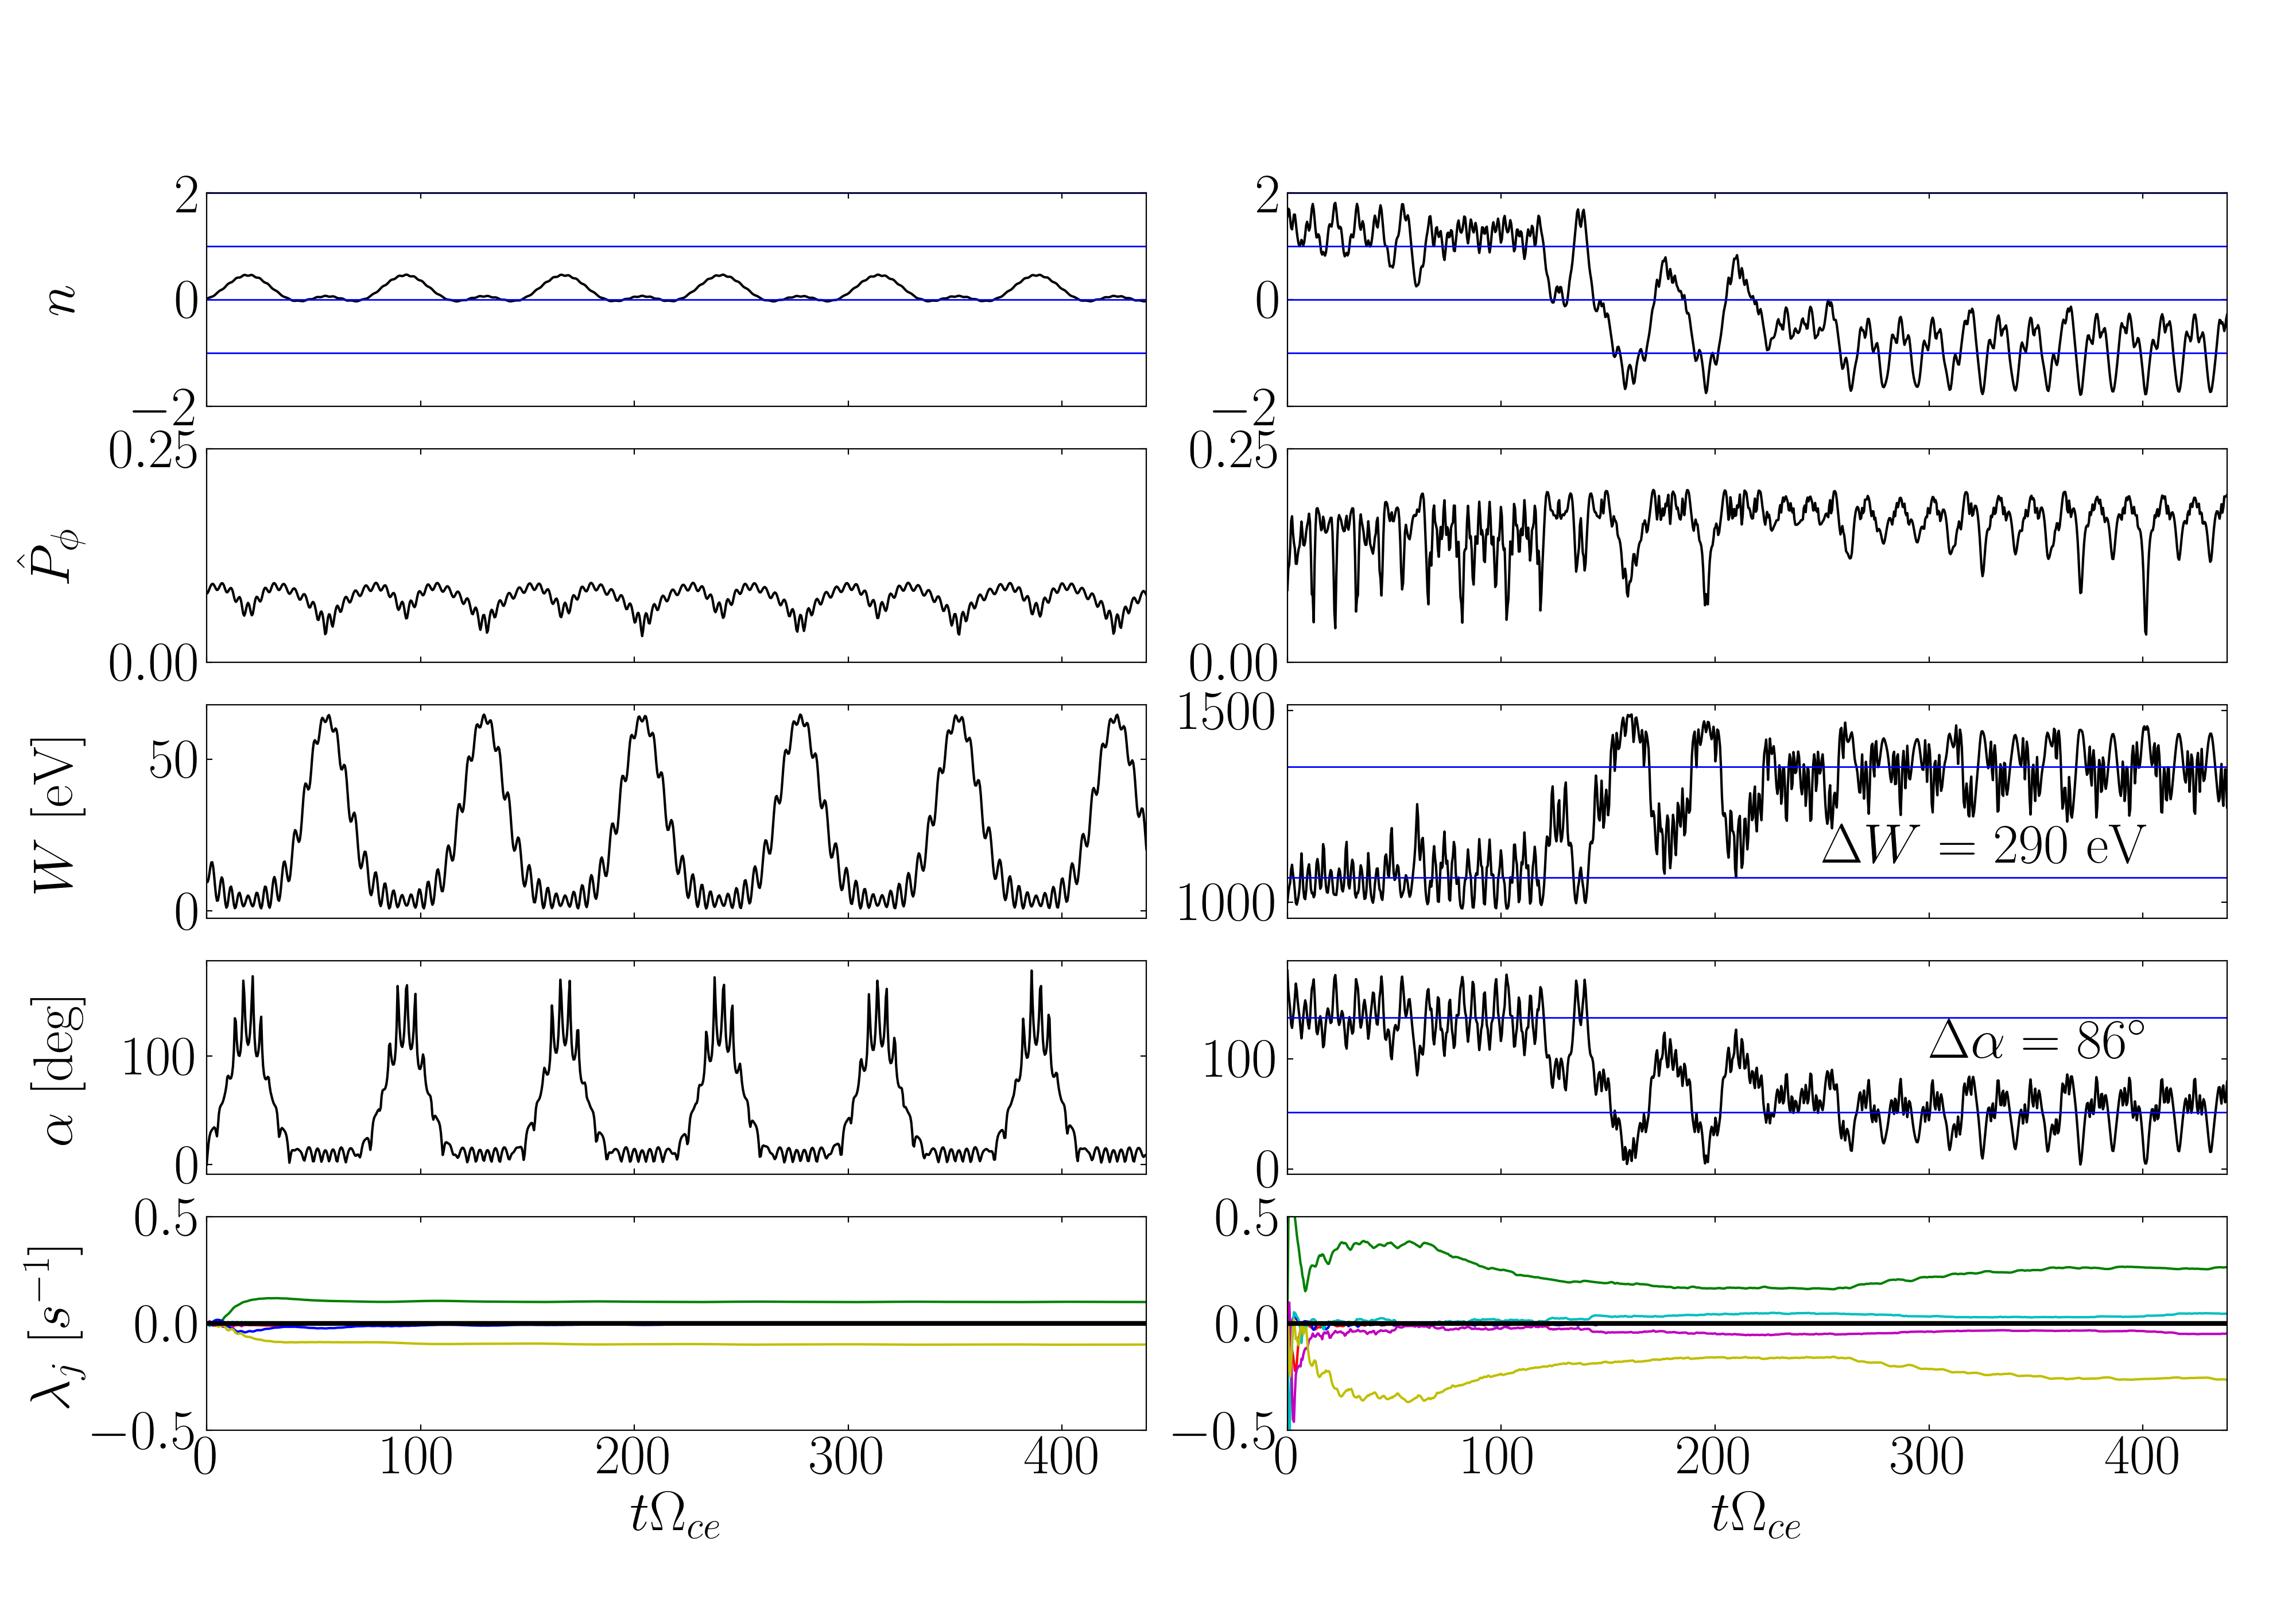
\includegraphics[width=\textwidth]{compare_time_series.png}
    \caption{Time series of two electrons with initial conditions
    $(W_0,\alpha_0)$ = (10\,\si{eV},0$^\circ$) (left column) and
    $(W_0,\alpha_0)$ = (1\,\si{keV},180$^\circ$) (right column) interacting with
a single 65$^\circ$ whistler at 1 AU. The first row shows the resonant mismatch
$n$ calculated from \cref{eq:resonant_condition}. The second row is the
adiabatic invariant $\hat{P_\phi}$ conjugate to the transformed gyrophase
$\phi$. The third row is the kinetic energy $W=(\gamma-1)mc^2$. The fourth row
is the pitch angle $\alpha=\cos^{-1}\qty(v_z/v)$. The last row shows the
Lyapunov exponent spectrum $\lambda_j$ in colors, each corresponds to one of
the six dimensions in the 6-ball, and the LCE in black.}
    \label{fig:compare_time_series}
\end{figure}

\cref{fig:compare_time_series} shows the dramatic differences in the response of
two particles. One is fast (1\,\si{keV}) and the other is fairly slow
(10\,\si{eV}).  For the slow particle, we can see quasi-periodic motion where it
enters the Landau resonance $(n=0)$ briefly, resulting in an energization in $W$
while the pitch angle $\alpha$ remains constant. Note that the adiabatic
invariant $\hat{P_\phi}=P_\phi-n\hat{P_\zeta}$ is modulated by $G_n\propto
\rho J_n'(k_\bot\rho)$ for small $P_\|$ and $\rho$ near the resonance. So for
the slow particle, the fluctuations in $\hat{P_\phi}$ are small ($\sim0.01$)
near $n=0$. For the 1\,\si{keV} particle, the energization and scattering is
much more significant. As it flips from $n=1$ (the fundamental cyclotron
resonance) to $n=-1$, the kinetic energy $W$ is increased by 30\% of its initial energy and it is scattered by $86^\circ$. It is also worth noticing that the particle sporadically enters and exits a resonance in a short time scale, leading to spikes of the order of $0.1$ in the adiabatic invariant.


From \cref{sec:particle_dynamics}, the particle's energy and
adiabatic invariant are not conserved when it crosses a resonance. So these
conservation laws are momentarily broken. However, in this non-relativistic
energy range ($W\sim1$\,\si{keV}), the resonance crossing occurs frequently and
sporadically, resulting in less distinctive changes than an example already
shown in \cref{fig:resonance_crossing}, which is typical of wave-particle interactions in the radiation belts. This is due to the small wave fields assumption in \cref{sec:particle_dynamics}. Specifically, it is required
that $\abs{qA/mu_{\max}}\ll 1$ for the radiation belts conditions to
apply. However, it is shown in
\cref{fig:potential_dominance}  that the initiated particles have maximum 
velocity $u_{\max}$ such that $\abs{qA/mu_{\max}}$ is $\sim\mathcal{O}(0.1)$. 
So the simulation of large amplitude whistler waves result in nonlinear effects 
much different from radiation belts context. For the sake of demonstration, a 
comparably similar behavior can be obtained by simulating relativistic 
electrons. \cref{fig:relativistic_resonance_crossing} shows the distinctive 
jumps in the resonant harmonic $n$ and the adiabatic invariant $\hat{P_\phi}$ 
for a 1\,\si{MeV} electron under the interaction of the same wave parameters as 
those in \cref{fig:compare_time_series}. Note that the trapping occurs both 
near a resonance and outside a resonance. A method to identify trapping
occurences has not yet been developed.

\begin{figure}[hbtp]
    \centering
    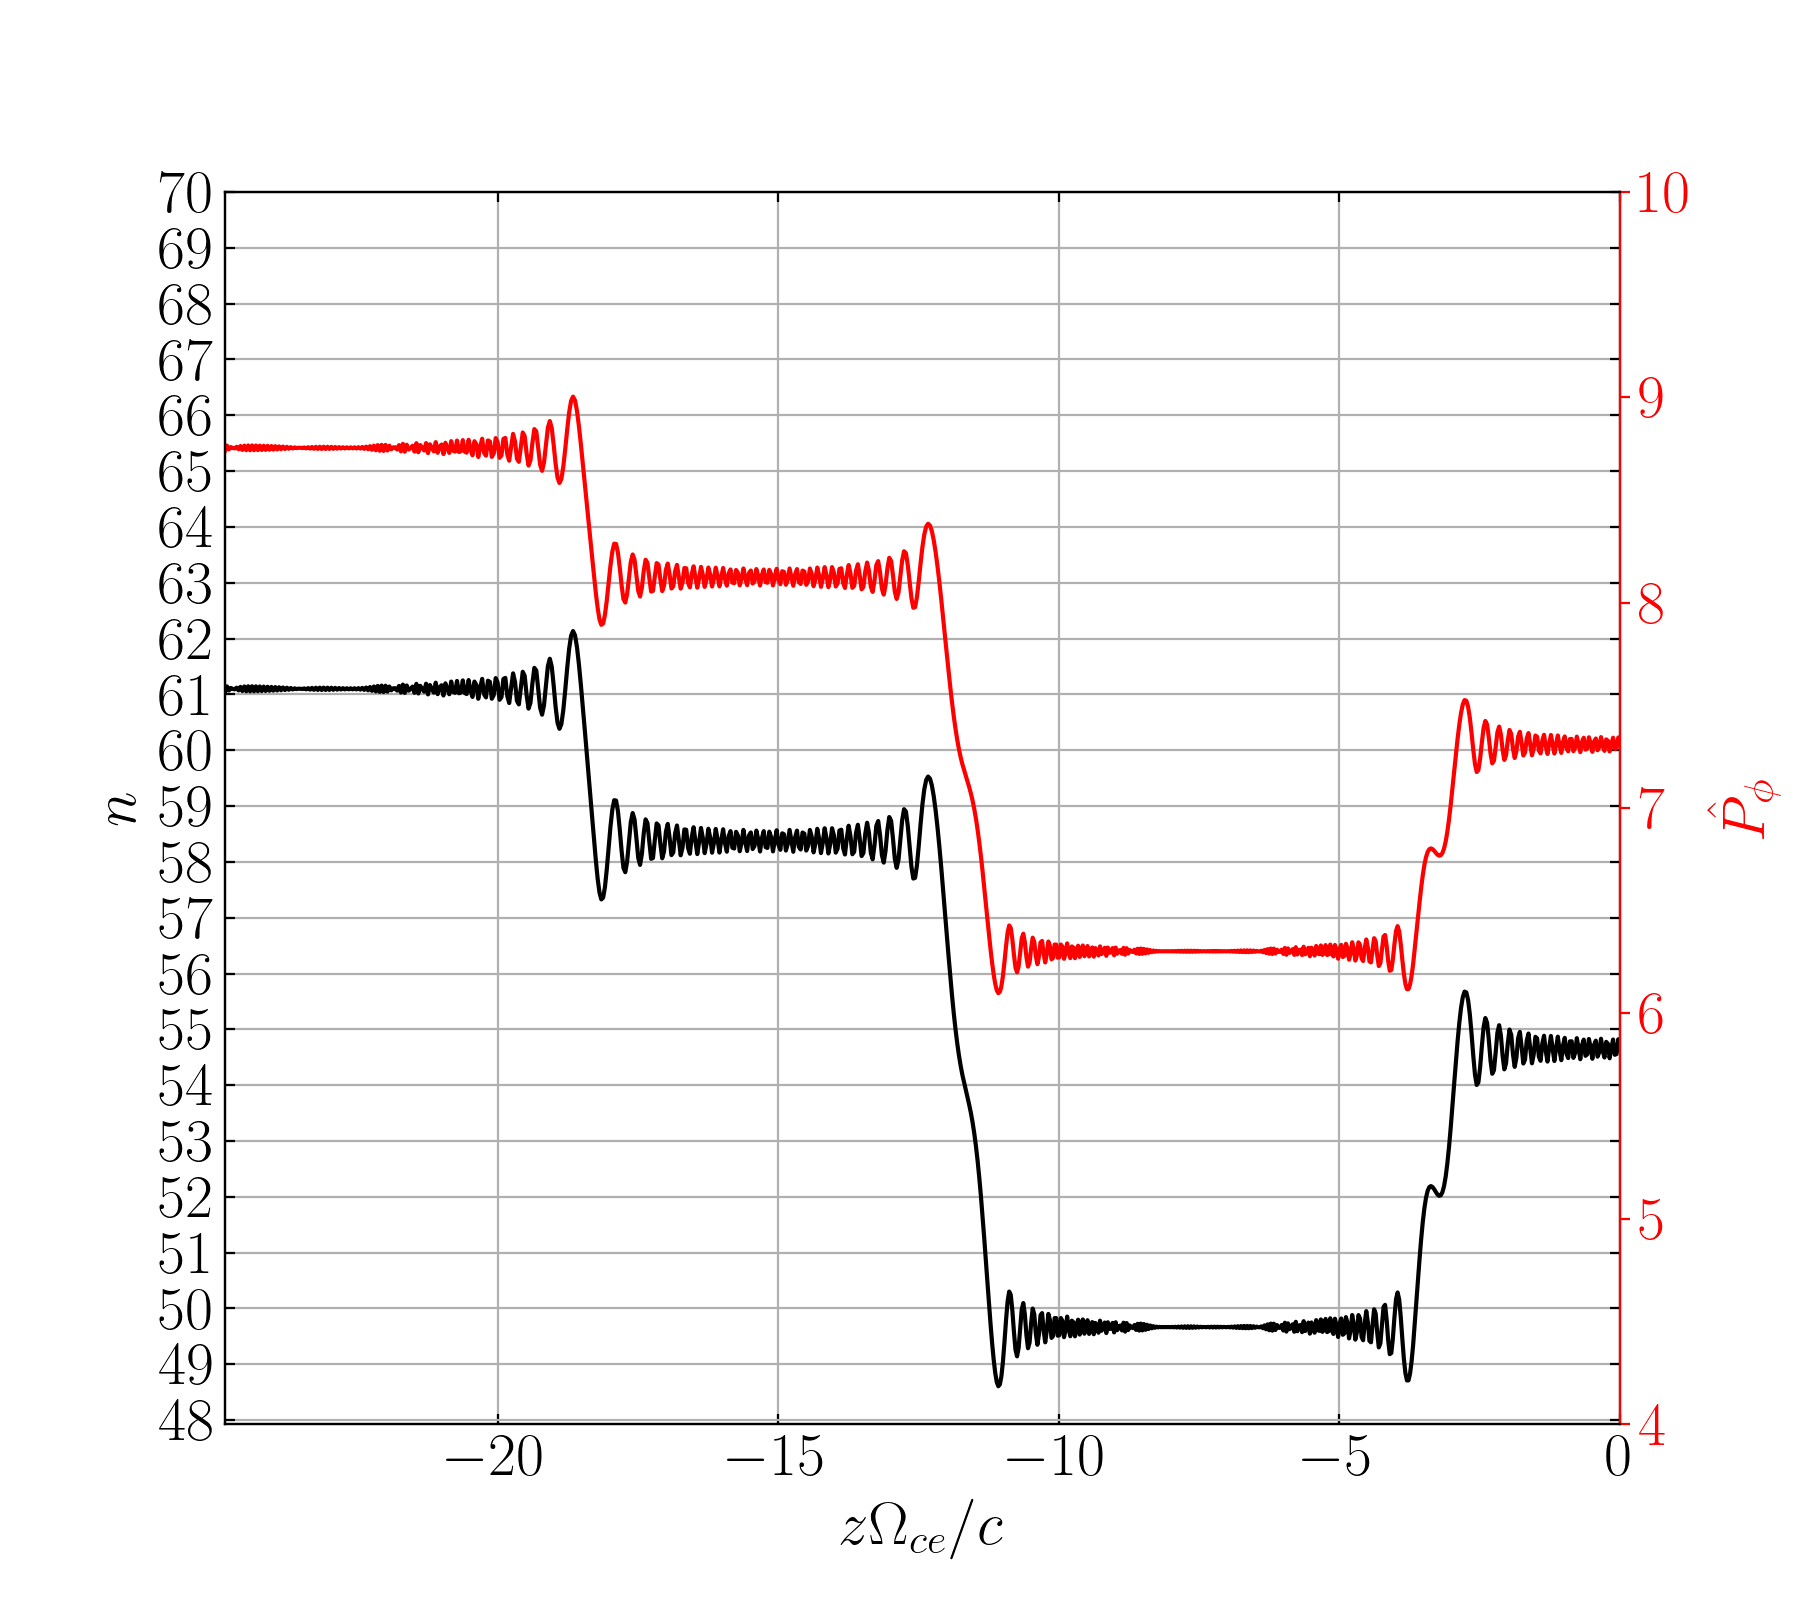
\includegraphics[width=0.7\textwidth]{diagnostics_resonance_crossing.png}
    \caption{Resonance crossing of a 1\,\si{MeV} particle interacting with a
    single 65$^\circ$ whistler at 1 AU. The left (black) axis plots the
resonance mismatch $n$, and the right (red) axis shows the adiabatic invariant
$\hat{P_\phi}$.}
    \label{fig:relativistic_resonance_crossing}
\end{figure}

The Lyapunov exponent spectrum, i.e., the different components $\lambda_j$, is
plotted in different colors in the last row of \cref{fig:compare_time_series}.
None of the components have any physical significance because the 6-D ball is free to rotate along the particle trajectory in our
calculations as described in \cref{sec:sim_LCE}. But they signify that there is
always at least one chaotic component, which corresponds to the sporadic
violation of the conservation of the adiabatic invariant inherent in our system.
Now, it is their sum, the LCE, that is important. As expected, the Lyapunov
exponents converge after a transient period at the beginning. So the estimation
of the LCE after a sufficiently long time period is constant. This enables the
estimation of the best step size to use without running very long simulations.
\cref{fig:LCE_compare} shows the LCE of all of the initiated particles after it
has reached convergence. The maximum LCE is $\lambda\sim10^{-3}$ in both cases.
Thus, for a step size of $\Delta t=10^{-4}$, the volume of the 6-D ball scales
as $\exp\qty(\lambda N\Delta t)\sim 1$ as long as the number of steps
$N\lesssim10^{7}$. In the physical parameters of interest, $10^7$ steps 
correspond to $\sim 60$ wave periods, which is a sufficiently long simulation 
time to study the responses.

\begin{figure}
    \centering
    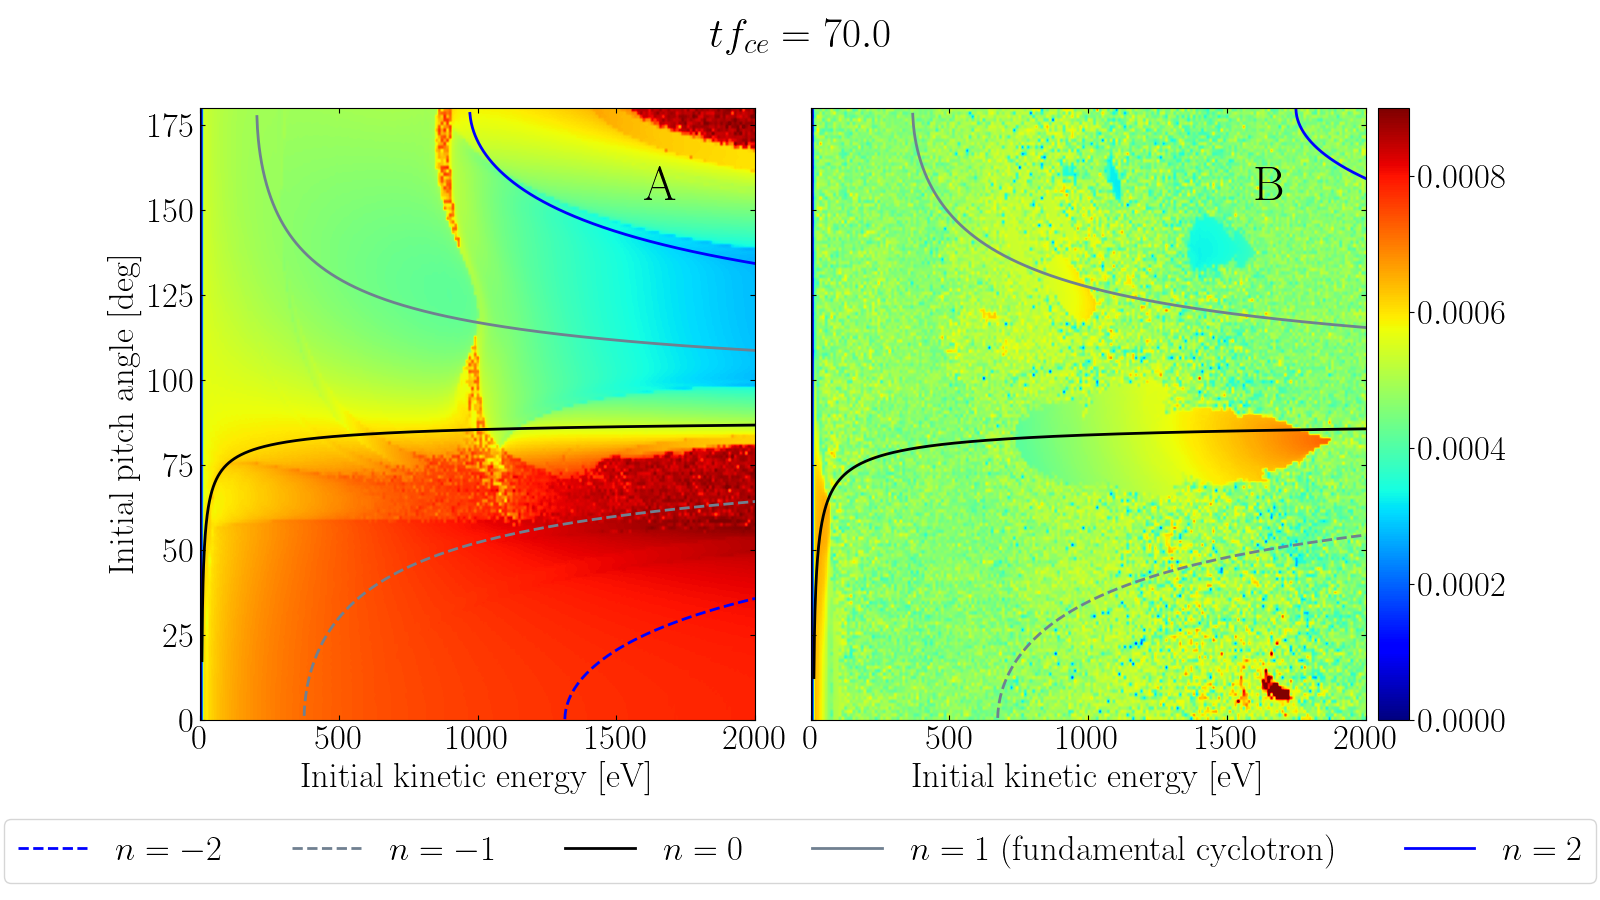
\includegraphics[width=\textwidth]{LCE_compare.png}
    \caption{The LCE of the simulations with a single $5^\circ$ whistler (A) and
    a single $65^\circ$ whistler (B) at 1 AU after a sufficient simulation
period for its convergence.}
\label{fig:LCE_compare}
\end{figure}


\section{Analysis}\label{sec:analysis}

In this section, we discuss the structure of the VDF after a long simulation
period (60 wave periods for 1 AU and 45 periods for 0.3 AU). In the case of 1 AU
parameters, the following figures will include the core, halo, strahl, and 
total distribution function, while in 0.3 AU parameters, the distribution 
includes only the core and strahl electrons. In this non-relativistic range of 
energy, the $R$ surfaces are almost straight lines, so only the 
intersections (white crosses) with the $v_\perp=0$ axis are plotted to signify 
their locations (as derived in
\cref{eq:resonant_velocity}). The concentric ellipses (black curves) are the
constant $H$ surfaces (from \cref{eq:constant_H_surface}), the center of which is the Landau resonance $(n=0)$. The intersections of the $H$ surfaces with the
$v_\perp=0$ axis show the $n=\pm1,\pm2,...$ radially from the $n=0$ mode. Recall
that in this work's convention, the $n<0$ modes are always along the parallel 
velocity range and the $n>0$ modes are along the anti-parallel range (as 
opposed to most papers in the literature).

\subsection{Single whistlers at 1 AU}
\begin{figure}
    \centering
    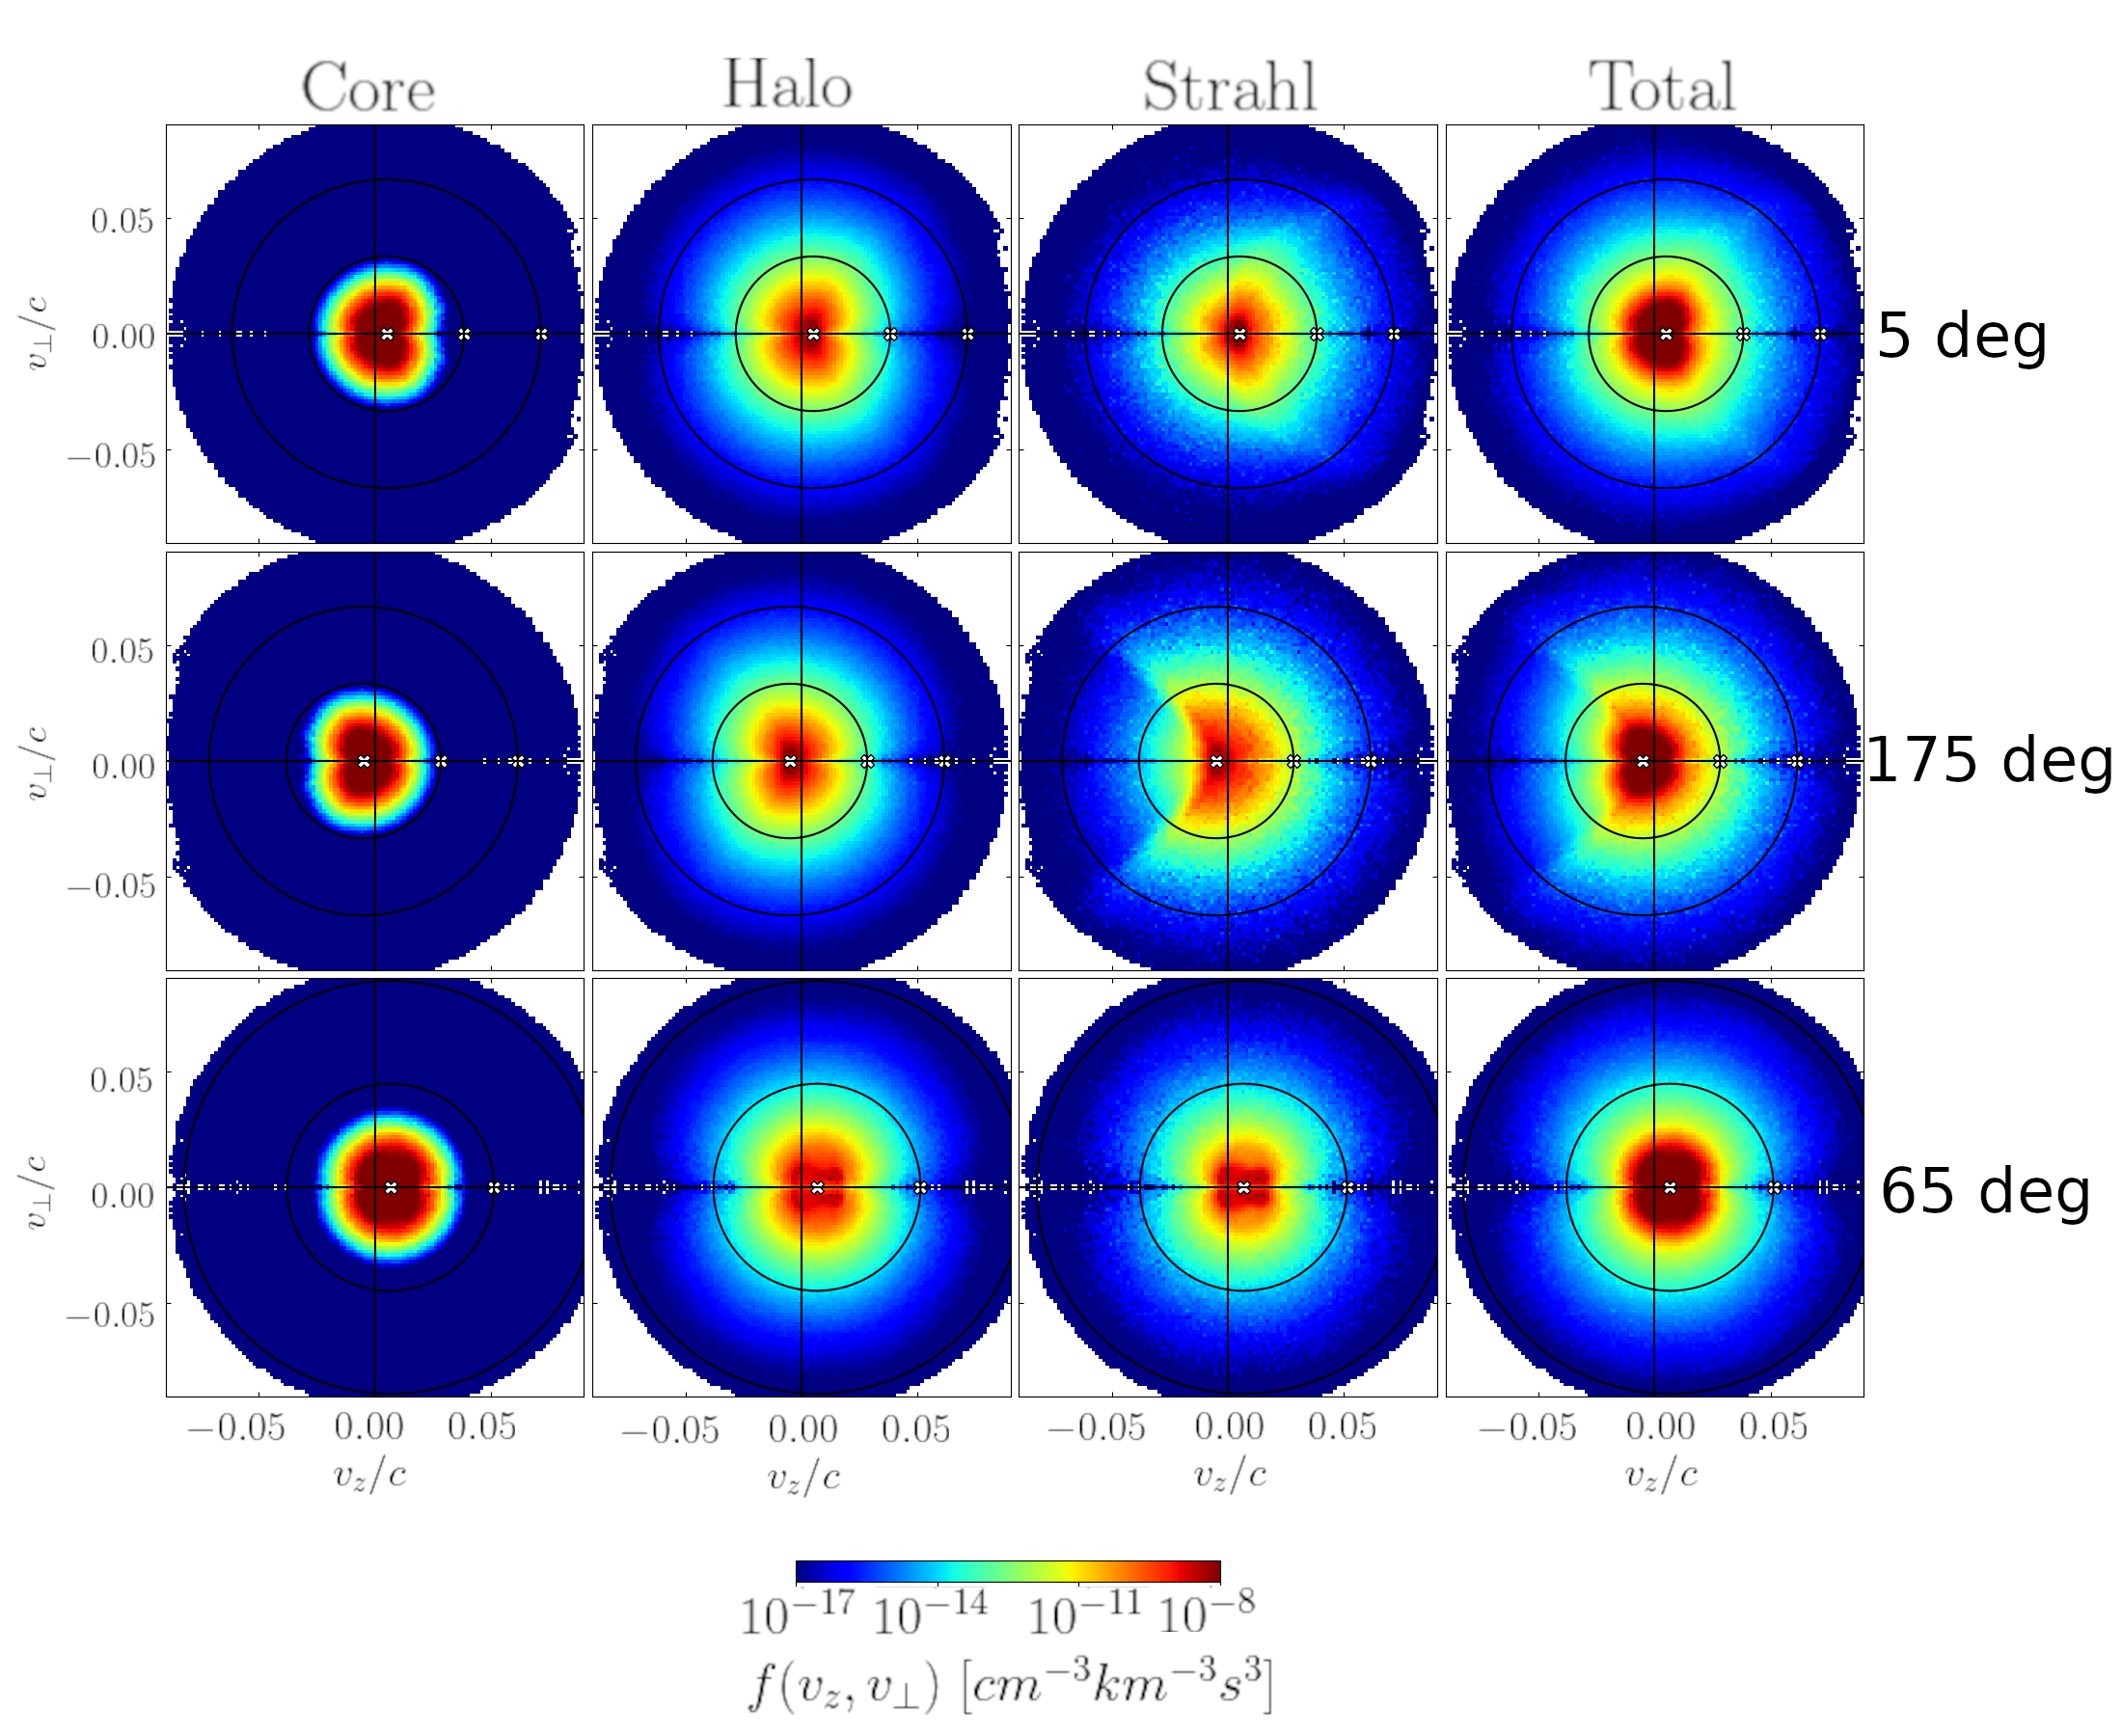
\includegraphics[width=\textwidth]{single_whistlers_1AU.png}
    \caption{VDF of electron populations after 60 wave periods of interaction
    with a single whistler at 1 AU. From top to bottom, the rows are the
simulations with the $5^\circ$, $175^\circ$, and $65^\circ$ wave.}
    \label{fig:single_whistlers_1AU}
\end{figure}

For single whistlers, \cref{fig:single_whistlers_1AU} shows the results from 
three simulations which demonstrate the interactions with (from
top to bottom) an almost parallel ($5^\circ$), an almost antiparallel
($175^\circ$), and an oblique ($65^\circ$) wave after 60 wave periods. The
final VDF of the two parallel cases approximately mirror each other, however,
the structures are not entirely identical since the background field points
along the wave in one case and against the wave in another, while the strahl
electrons are propagating along the field. The first two rows
indicate that parallel waves are able to scatter electrons to a certain extent.
However, there is a prominent bow-like feature near the $n=-1$ mode at an angle
of $\sim50^\circ$ around the $v_\perp=0$ axis, which is most apparent for the
anti-parallel case. The last row indicates that the interaction with an oblique
whistler efficiently isotropizes the strahl, which results in a structure
almost identical to the halo by the end of the simulation period. However, there
is a lack of high energy and parallel propagating particles, which has been
observed in the energy-pitch angle distribution in PSP data
\citep{Cattell2021b}. This makes the final results not completely isotropic.
Thus, it is not suitable to apply the fitting procedure for the model
defined in \cref{eq:kappa} that \cite{Wilson2019} used for satellite observations of the VDF.

To better understand the VDF structures, the
trajectories of a few particles interacting with the 5$^\circ$ and
65$^\circ$ waves during the entire simulation period are shown in \cref{fig:single_O5_1_AU}. In panels A1, B1, C1, and D1, the particles move along their corresponding $H$
surfaces as expected. The corresponding histograms (A2, B2, C2, and D2) show the
points along the particle's trajectory where they hover around the most. In the
interaction with the 5$^\circ$ wave (panels A and B), the histograms are uniform, indicating that the particles bounce back and forth in a quasi-periodic motion. There is a point of ``reflection'' for each energy, which results in the bow-like feature in the VDF. These points are close to the intersections of the $H$ surfaces and the $n<0$ resonances. This can be due to a combined effect of (a) magnetic mirroring due to the large wave fields comparable to the ambient field and (b) resonant interaction. Effect (a) is a speculation that needs further analysis beyond the scope of this thesis. Here we shall only offer an explanation for (b) from the theory of resonance derived in \cref{sec:theory}.

For $n<0$, the electron overtakes the wave when it observes a left-hand polarized electromagnetic field in its own frame. Thus, being a right-hand particle, it no longer interacts resonantly. This results in the deceleration of $v_z$ to the negative range where resonant interaction is enabled once again because the particle observes a right-hand polarized wave. It would be interesting to study whether this occurs for a self-consistently simulated wave-particle interaction using PIC code. This is because the $n<0$ modes are usually where the particle transfers its energy to the wave as it rotates out of phase with the fields, leading to wave generation instead of damping \citep{Tsurutani1997}. Thus, the wave is modified due to this type of quasi-parallel whistler heat-flux instability \citep{RobergClark2019,Micera2020} and both the $H$ and $R$ surfaces are altered accordingly. This might allow the VDF to become more isotropic for particles under interactions with parallel whistlers.

\begin{figure}[hbtp]
    \centering
    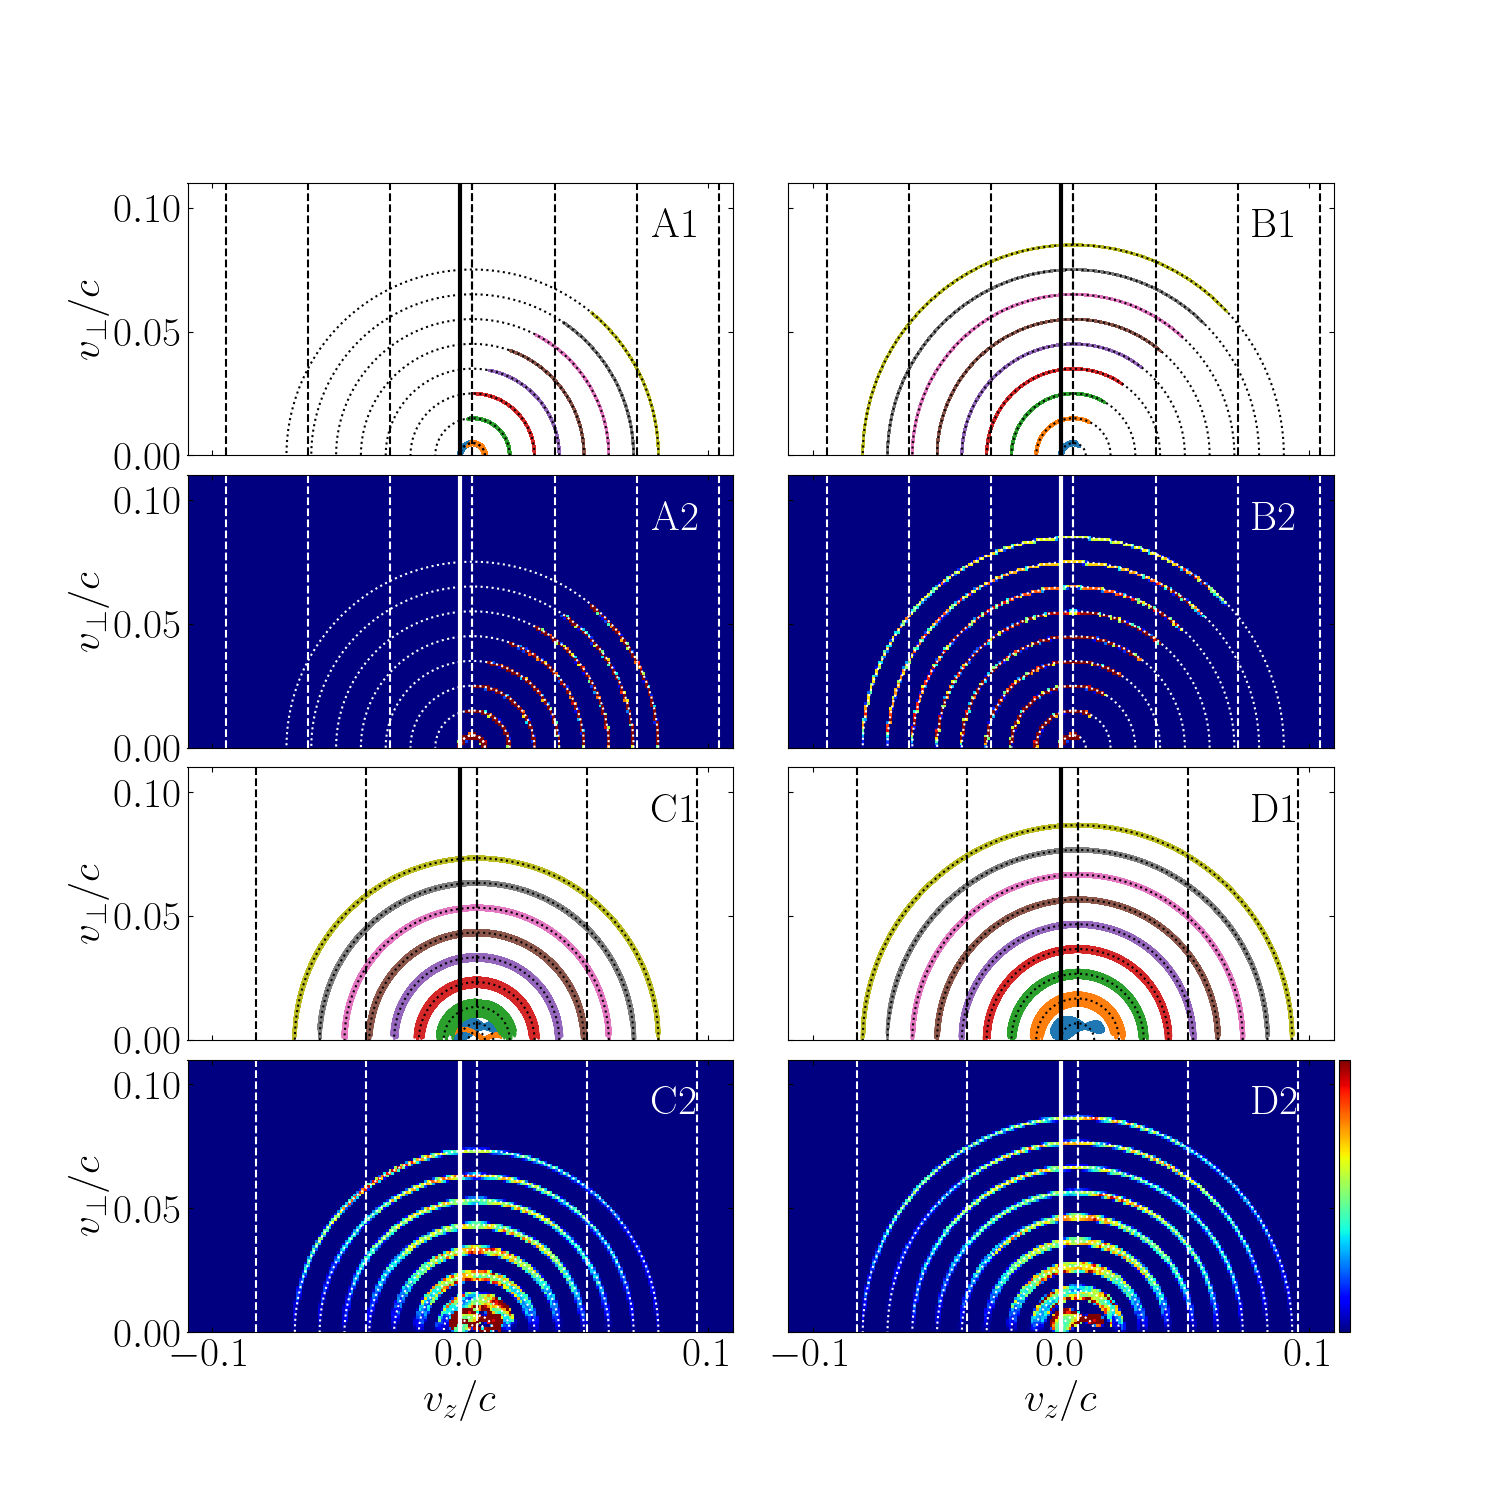
\includegraphics[width=\textwidth]{single_combo_trajectory.png}
    \caption{Traces of electron trajectories in the entire simulation period
        (1 AU parameters) and
        their corresponding histograms. The panels show those for electrons that are originally parallel (A1-A2) and antiparallel (B1-B2) to the
        single 5$^\circ$ whistler. Similarly, (C1-C2) and (D1-D2) are those
        parallel and antiparallel to the single 65$^\circ$ whistler. Their
    initial speeds are $0,0.01,0.02,...,0.08c$, which correspond to
$0,26,102,...1643$\,\si{eV}. The dotted curves are the constant $H$ ellipses
corresponding to the particle's intitial energy, while the dashed straight lines
are the $R$ surfaces corresponding to (from left to right) $n=3,2,...,-3$. The
solid lines are the $v_z=0$ axis.}
        \label{fig:single_O5_1_AU}
\end{figure}

Because the polarization for an oblique wave is elliptical, it is a
combination of both right-hand and left-hand waves. This allows for anomalous
interactions to occur, which happens when an electron (right-hand) interacts
with the $n>0$ harmonics of a left-hand wave by overtaking it
and observing a right-hand polarized electromagnetic field
\citep{Tsurutani1997}. Consequently, the scattering of electrons is more
isotropic in panels C and D, where both parallel and anti-parallel particles behave similarly.

\begin{figure}
    \centering
    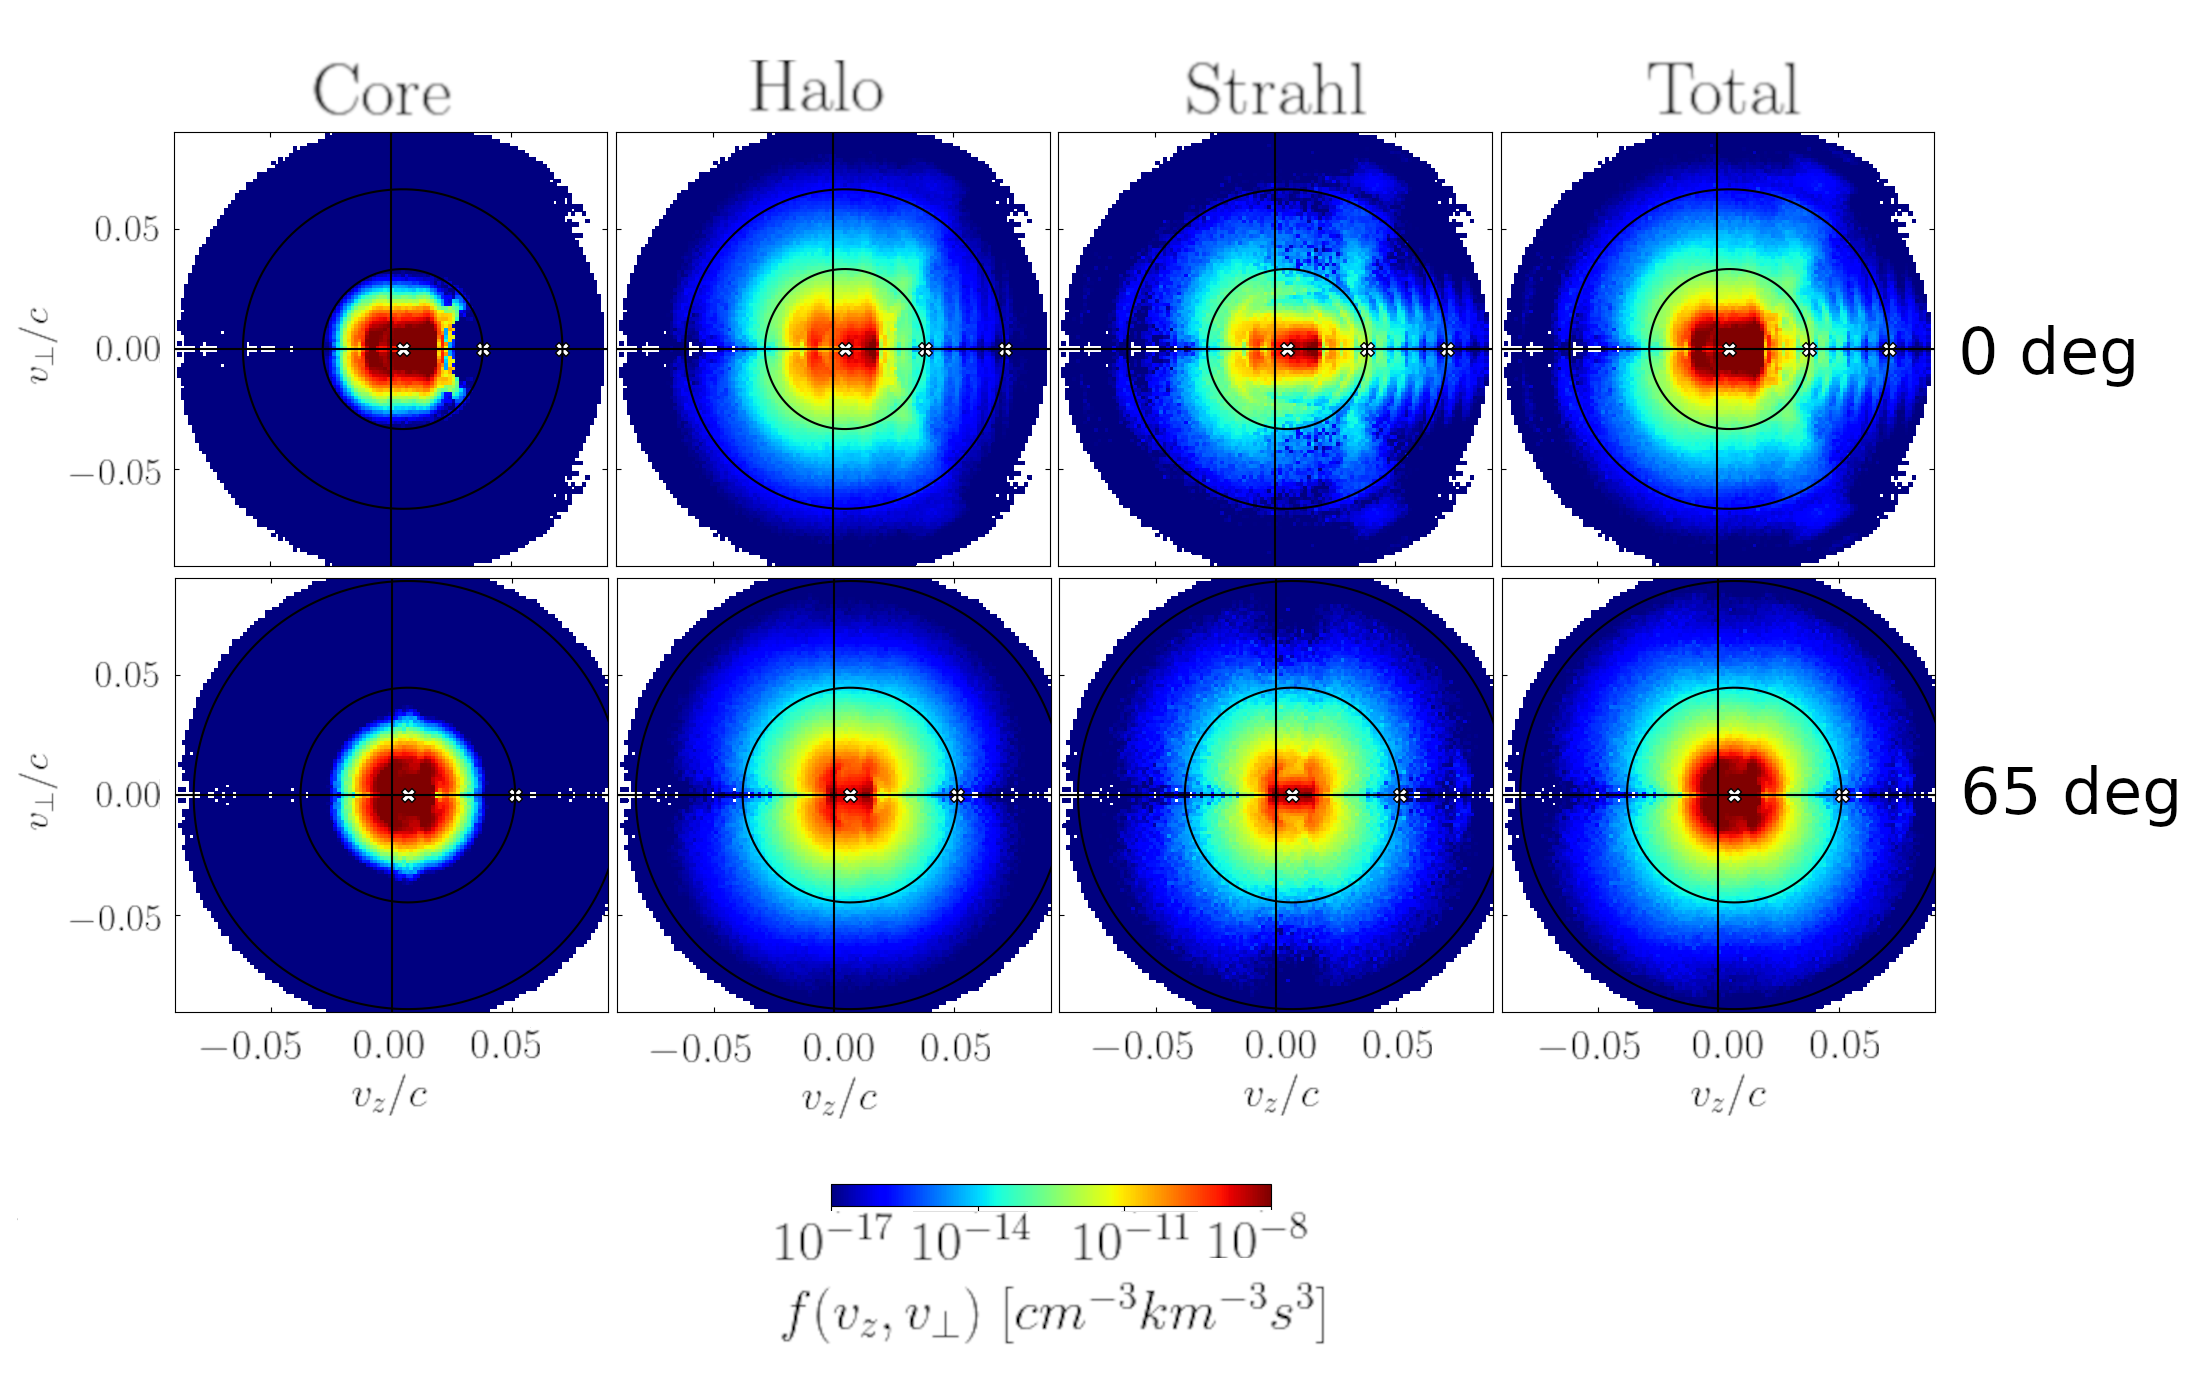
\includegraphics[width=\textwidth]{whistler_packets_1AU.png}
    \caption{VDF of electron populations after 60 wave periods of interaction
        with a $0^\circ$ (top row) and 65$^\circ$ (bottom row) whistler packet at 1 AU.}
\label{fig:whistler_packets_1AU}
\end{figure}

\subsection{Whistler packets at 1 AU}


\cref{fig:whistler_packets_1AU} shows the final VDF after 60 wave periods of
interaction with a $0^\circ$ packet and a $65^\circ$ packet in 1 AU parameters. A region of particle loss similar to that in the single wave parallel whistlers in the previous section can be seen in the $0^\circ$ packet. However, in addition to the bow-like region, there is also a vertical structure near the $n=-1$ harmonic. Because multiple frequencies are contained in the packet, the $R$ surfaces are now clustered. \cref{fig:packet_O0_1_AU} shows the surfaces corresponding to the packet's mean frequency wave. In panel B2, there are electrons trapped around the $n=-1$ cluster of $R$ surfaces. Those particles are energetic enough to enter the envelope of the cluster but they cannot escape, resulting in this vertical structure in the VDF. This further supports the explanation from the theory of resonance. In the frame of the mean-frequency
wave, there are other waves of different frequencies, which move in both
directions with respect to it. Their combined effects cause the trapping
around $n=-1$. However, large amplitude waves at $0^\circ$ are not seen in
the solar wind at 1 AU. The large amplitude waves at 1 AU are oblique, like the
$65^\circ$ packet. For this case, the electron interaction with the packet
is similar to the case of a single whistler for the strahl.

\begin{figure}[hbtp]
    \centering
    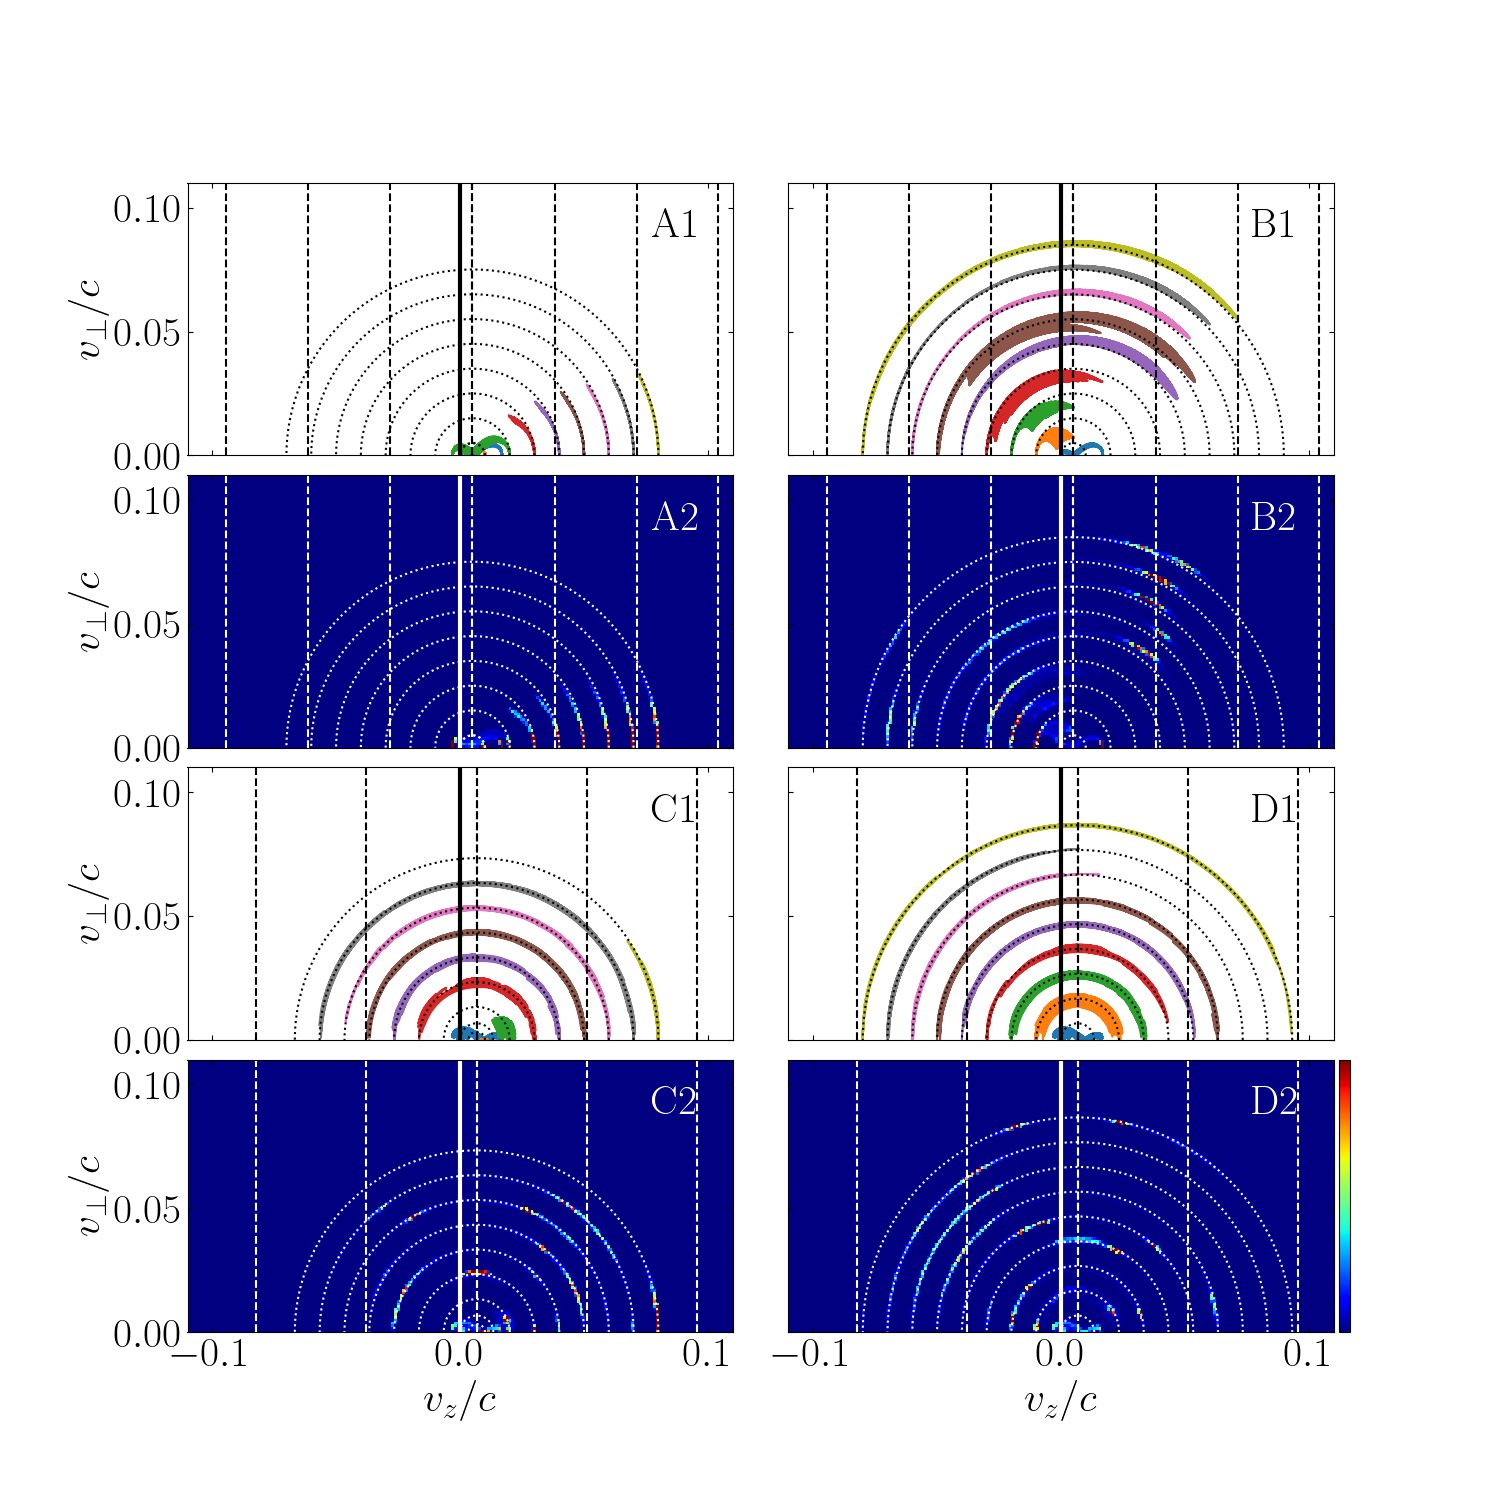
\includegraphics[width=\textwidth]{packet_combo_trajectory.png}
    \caption{Traces of electron trajectories in the entire simulation period
        (1 AU parameters) and their corresponding histograms. The panels are
        similar to those in \cref{fig:single_O5_1_AU}, but the electrons are
        under interactions with a 0$^\circ$ packet (A and B) and a 65$^\circ$
        packet (C and D).}
    \label{fig:packet_O0_1_AU}
\end{figure}

The scattering of particles interacting with the oblique packet is highly
localized and often in between the resonances (see panels C2 and D2). This is
most likely due to the overlapping resonance widths associated with each mode
\citep{Karimabadi1990}. In this work, the single-wave resonance surfaces are
spaced fairly closely between each harmonic $n$. The overlap of resonance widths
can cause more nonlinear and complicated interactions to occur. The calculation
of the widths is beyond the scope of this thesis.

\subsection{Whistler packets at 0.3 AU}

\begin{figure}[hbtp]
    \centering
    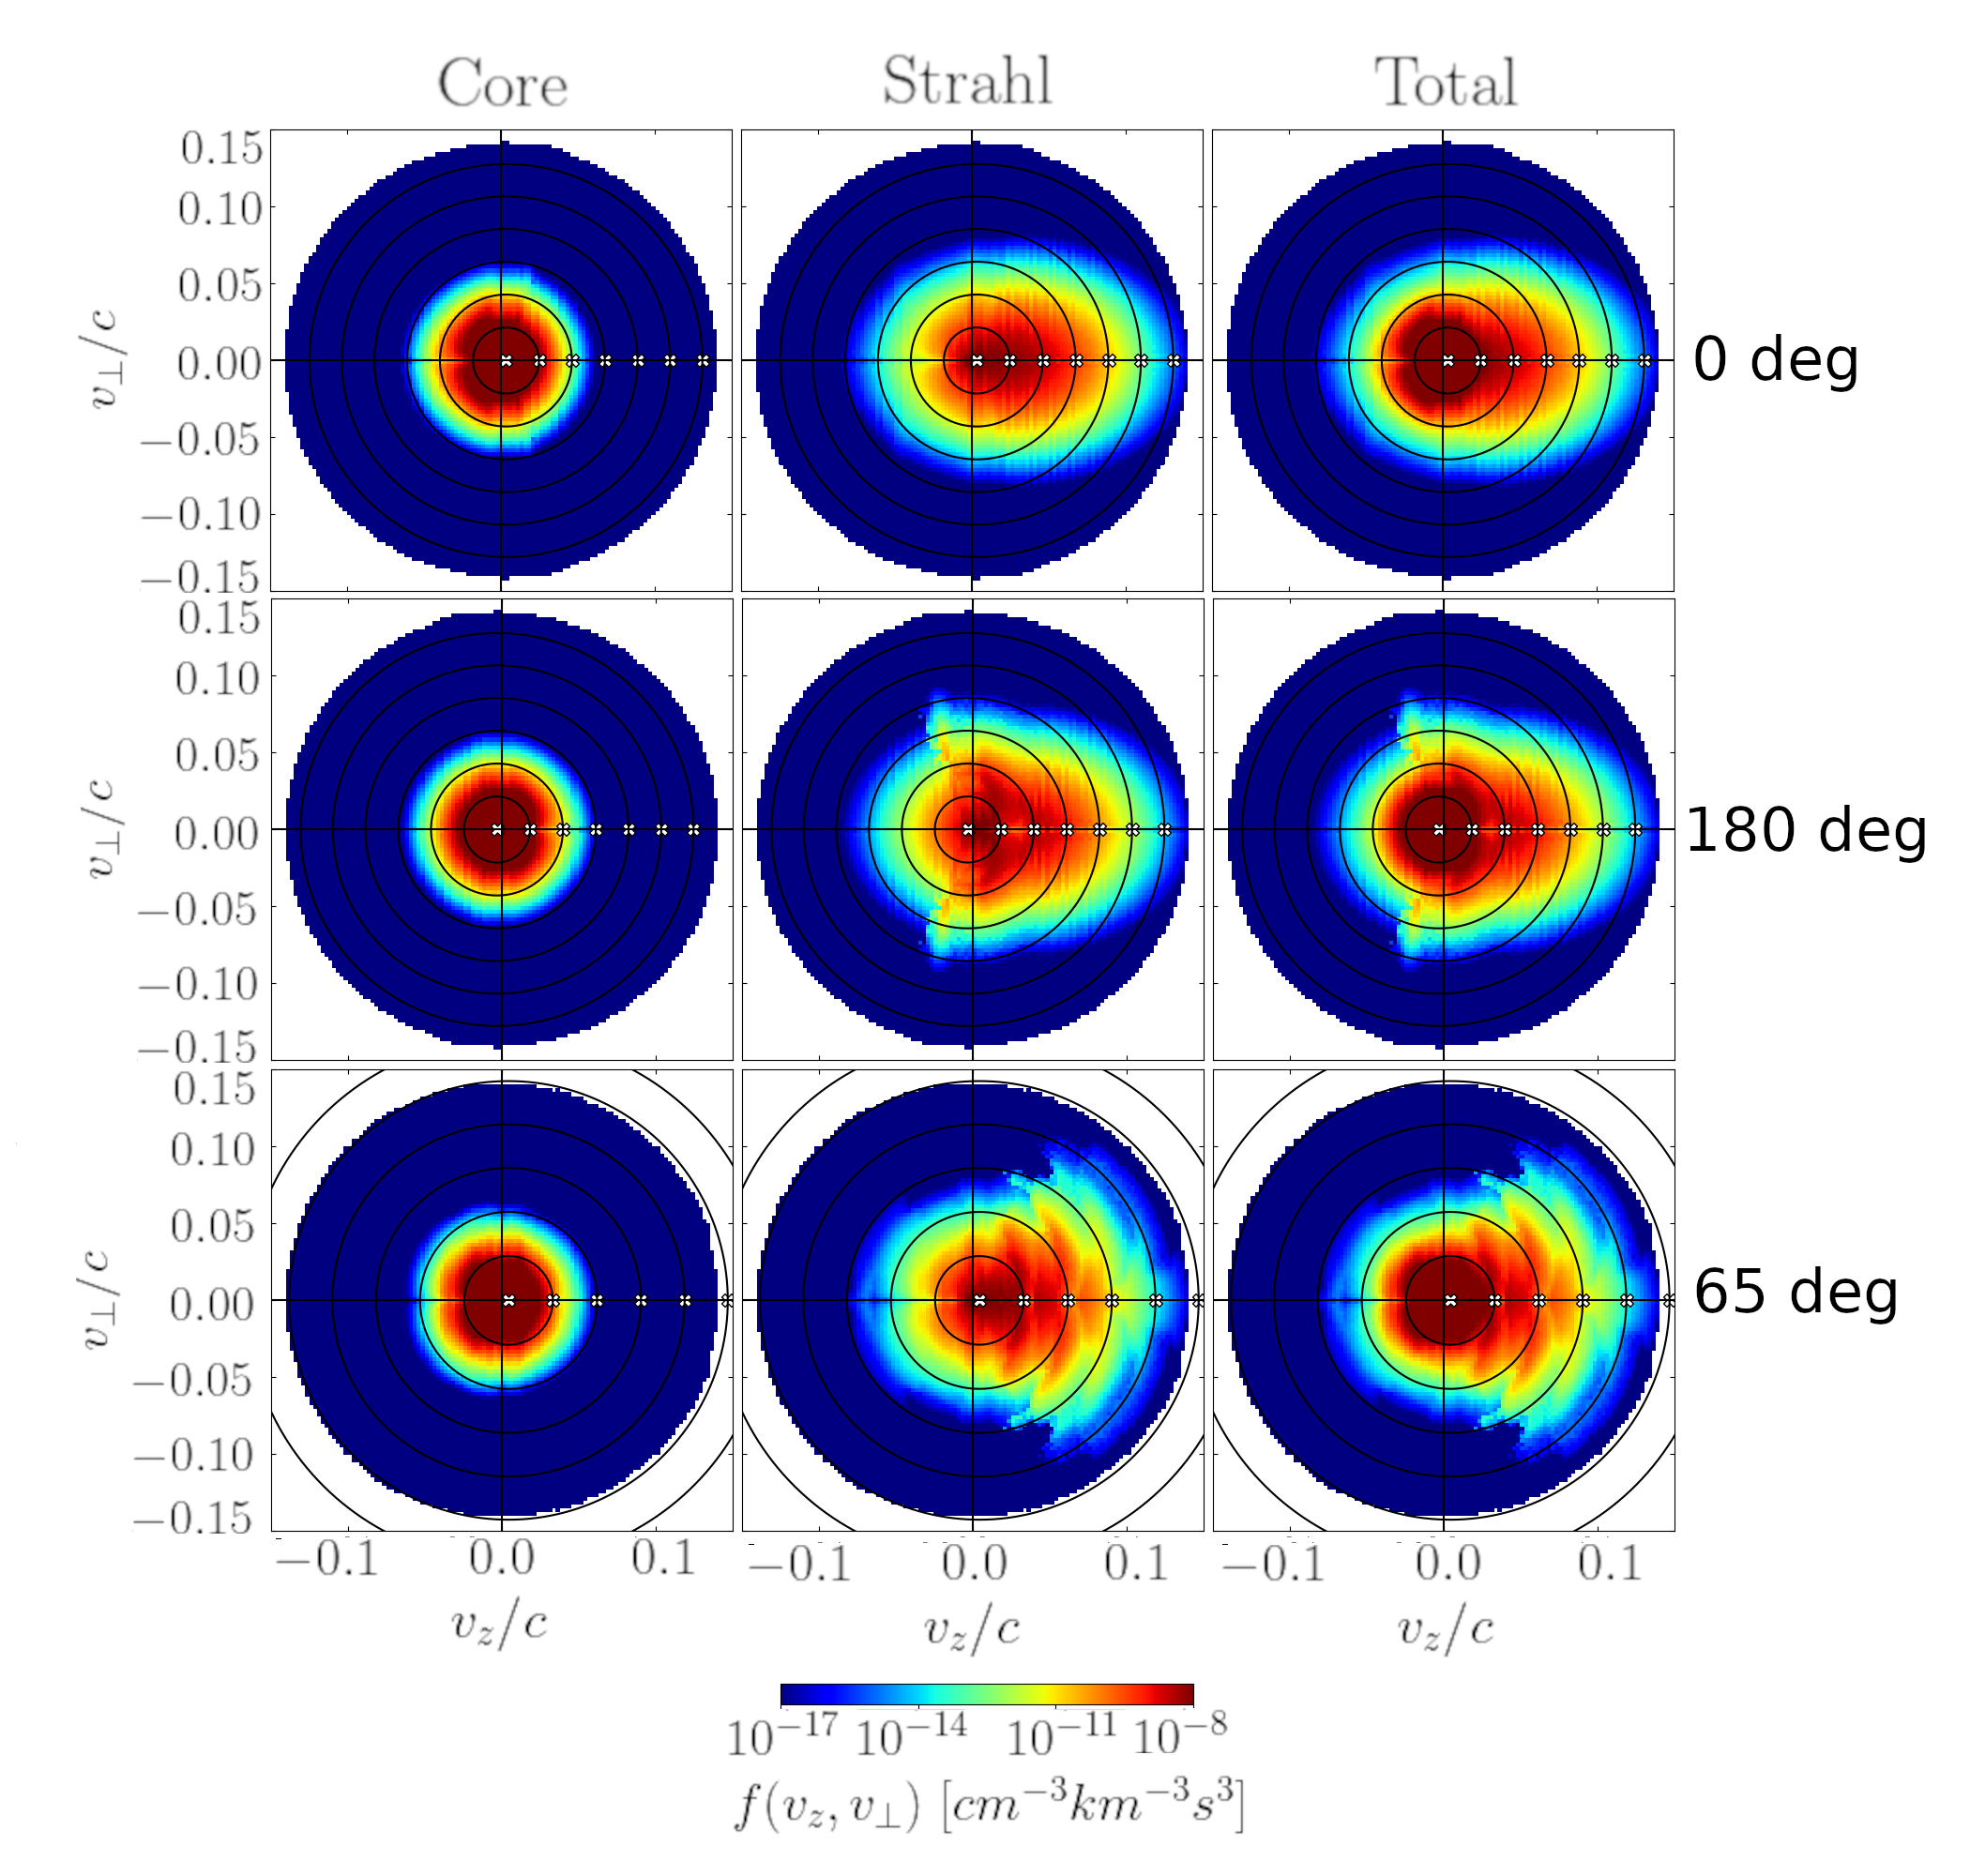
\includegraphics[width=\textwidth]{whistler_packets_03AU.png}
    \caption{VDF of electron populations after 45 wave periods of interaction
    with whistler packets at 0.3 AU. From top to bottom, the rows are the
simulations with the $0^\circ$, $180^\circ$, and $65^\circ$ wave.}
\label{fig:whistler_packets_03AU}
\end{figure}

For interactions with whistler packets in 0.3 AU parameters, we observe the
formation of ``horn''-like features in the VDF at the locations of the
$R$ intersections in the case of oblique propagation (see
\cref{fig:whistler_packets_03AU}). This is similar to what was reported in
\cite{RobergClark2019}. However, they studied very relativistic
electrons, which resulted in more defined horn features as the particle velocity
term dominates in the canonical momentum. In the discussed parameters, this 
dominance is weaker, which results in broader horns. Parallel packets do not 
scatter the strahl as efficiently as oblique packets near the Sun,
as similar to the discussion in \cite{Vocks2005}. \cite{Halekas2020b} reported
that the heat flux observed at 0.3 AU was consistent with the threshold for
oblique whistler fan instability. So these results are consistent with near-Sun 
observations.






\section{Conclusion}\label{sec:conclusion}
A vectorized test particle simulation is used to study the scattering and
energization of solar wind electrons from their interactions with single
whistlers and whistler packets at different propagation angles and in 0.3 AU and
1 AU background parameters. It is shown that for non-relativistic particles, 
the interaction is mainly a diffusion in pitch angle. The particles are 
scattered along the constant $H$ surface while interacting with the nearest 
resonant mode. The presented results show that the final velocity distribution 
function at 0.3 AU is consistent with observations from PSP 
\citep{Cattell2021b,Halekas2020b} and with simulations in 
\cite{RobergClark2019} and \cite{Micera2020} for the case of obliquely 
propagating whistler packets. Resonant strahl electrons are scattered to a 
higher pitch angle until they can be characterized as an isotropic halo. This verifies the theory that the origin of the halo is
the strahl, since these waves can scatter the VDF in a short length scale. Thus,
it explains the existence of a halo population of electrons far from the Sun at
1 AU and the corresponding heliospheric radial decrease in strahl density. It is
also observed that parallel waves are less efficient in isotropizing the
electron distribution, consistent with the heat-flux study in \cite{Halekas2020b}.


\section{Future works}\label{sec:future_works}

Much of the analysis can be further extended from the basis laid out in this
thesis using the Hamiltonian approach. The resonance widths of the
harmonics can be calculated to determine the overlapping and their subsequent
effects on the VDF structure. Since the derived adiabatic invariants are
analogous to the magnetic moment for a system without the wave perturbations,
they can be used to determine the constraints on the velocity, which describes
the magnetic mirroring effect. More interesting physics might be revealed by
simulations of the interaction of relativistic electrons with the large
amplitude waves described in this thesis. This is because the small field
assumptions of $\delta_{1,2}$ are better satisfied if the particle momentum term
dominates in the canonical momentum. In terms of the simulation program, the
developed code is written purely in Python and is vectorized with Python arrays, but better optimization can be achieved with true SIMD vectorization in C. This simulation program might be further developed into a full PIC code with the implementation of field solving components, in which case, a translation to C is absolutely necessary.



\newpage
\appendix
\appendixpage

\section{Useful mathematical theorems}

\begin{theorem}[Leibniz's integral rule]\label{thm:leibniz_rule}
    Given a bounded domain $I\subseteq\R$ with bounded boundaries $a(x),b(x)$
    defined on $I$, let $f(x,t)$ be a $C^1$ smooth function on
    $I\times\qty[a(x),b(x)]$. Also, suppose $a,b$ are $C^1$ smooth. Then for
    $x\in I$,
    \begin{equation}
        \frac{d}{dx}\qty(\int_{a(x)}^{b(x)}f(x,t)dt)=f(x,b(x))\cdot
        \frac{db(x)}{dx}-f(x,a(x))\cdot\frac{da(x)}{dx}+\int_{a(x)}^{b(x)}\frac{\partial
        f(x,t)}{\partial x}dt
    \end{equation}
\end{theorem}

\begin{theorem}[Bessel decomposition]\label{thm:bessel_decomposition}
    For $x\in\R^+$ and $\phi,\delta\in\R$, the following sinusoidal functions
    with oscillatory phase can be decomposed into Bessel-Fourier series
    \begin{subequations}
        \begin{align}
        \sin\qty(x\sin\phi+\delta)&=\sum_{n\in\Z}J_n(x)\sin\qty(n\phi+\delta)\\
    \cos\phi
        \sin\qty(x\sin\phi+\delta)&=\sum_{n\in\Z}\frac{n}{x}J_n(x)\sin\qty(n\phi+\delta)\\
        \sin\phi\cos\qty(x\sin\phi+\delta)&=\sum_{n\in\Z}J_n'(x)\sin\qty(n\phi+\delta)
        \end{align}
    \end{subequations}
    where $J_n(x)$ are the $n$th order Bessel functions of the first kind and
    $J_n'(x)$ are their first order derivative.
\end{theorem}

\section{The Hamiltonian resonance
analysis}\label{sec:hamiltonian_analysis}

In this section, we perform two transformations to reduce the Hamiltonian in
\cref{eq:relativistic_hamiltonian} into an integrable 1-D form, from which the
adiabatic invariants can be calculated and the resonant condition is derived
from the equation of motion. Assuming that the wave fields are small, we can
write $\HH=\HH_0+\HH_1$ in a power series of $A_1$ and $A_2$ to the first order
as follows. \begin{equation}\label{eq:Hamiltonian_original_form} \HH= \gamma
mc^2 -\frac{qA_1}{\gamma m}\qty[\qty(\frac{k_\parallel}{k})P_x-\qty(\frac{k_\bot}{k})P_z]\sin\psi -\frac{qA_2}{\gamma m}\qty(P_y-qB_0x)\cos\psi +q\Phi_0\sin\psi \end{equation}
where $\HH_0=\gamma mc^2$ is the Hamiltonian without the presence of any wave
and
\begin{equation}
    \gamma=\sqrt{ 1 +\frac{P_x^2}{m^2c^2}
        +\frac{(P_y-qB_0x)^2}{m^2c^2} +\frac{P_z^2}{m^2c^2} }
\end{equation}
is the Lorentz factor. From $\HH_0$, we can invert and
solve for $P_x$ \begin{equation}\label{eq:simplified_px}
P_x=\abs{q}B_0\sqrt{\frac{\HH_0^2/c^2-m^2c^2-P_z^2}{q^2B_0^2}-(x-X)^2}
=\abs{q}B_0\sqrt{\rho^2-(x-X)^2}
\end{equation}
where we have written
$X=P_y/qB_0$ and $\rho$ such that
$\HH_0=\sqrt{m^2c^4+q^2B_0^2\rho^2c^2+P_z^2c^2}$. Now, define the action
$J=(1/2\pi)\oint P_xdx=\abs{q}B_0\rho^2/2$,
which is just the area of a circle with radius
$\rho$ centered at $x=X$. Let $2\abs{q}B_0J=P_\perp^2$ and
$P_z=P_\parallel$.  The Hamiltonian then becomes
\begin{equation}\label{eq:x_independent_H0}
\HH_0=\sqrt{m^2c^4+2\abs{q}B_0Jc^2+P_\parallel^2c^2}=\sqrt{m^2c^4+P_\bot^2c^2+P_\parallel^2c^2}
\end{equation} $J$ is thus analogous to the perpendicular momentum and we can
interpret $\rho=P_\perp/\abs{q}B_0=v_\perp/\Omega_{c}$ as the particle's
gyroradius where $\Omega_c=\abs{q}B_0/m$ is the cyclotron frequency. \cref{eq:x_independent_H0} is now independent of the conjugate
coordinates. Thus, if we define the new momentum as $P_\phi=J$, then it is an
adiabatic invariant.

Now, we need to find the coordinate conjugate to $P_\phi$. Define the generating function
$F_2(x,y,z;P_\phi',P_y',P_\parallel')=\int_X^xd\overline{x}P_x(\overline{x};P_\phi',P_y')+yP_y'+zP_\parallel'$
where new variables are denoted with a prime. The old momenta transform
trivially as \begin{align} P_x&=\frac{\partial F_2}{\partial x}=P_x, &
P_y&=\frac{\partial F_2}{\partial y}=P_y', & P_\parallel&=\frac{\partial
F_2}{\partial z}=P_\parallel' \end{align} where the first equation is true due
to the First Fundamental Theorem of Calculus. The new $z$ coordinate can also be
found easily $z'=\partial F_2/\partial P_\parallel'=z$. Now, the coordinate
conjugate to $P_\phi'$ is given by \begin{equation}\label{eq:phi}
    \phi'=\frac{\partial F_2}{\partial P_\phi'}
=\int_X^x\frac{d\overline{x}}{\sqrt{\rho^2-(\overline{x}-X)^2}}
=\sin^{-1}\qty(\frac{x-X}{\rho}) \end{equation} Inverting, we get
$x=X+\rho\sin\phi'$. This simplifies the momentum $P_x$ in
\cref{eq:simplified_px} to $P_x=\abs{q}B_0\rho\cos\phi'$. Similarly, the new $y$
coordinate is \begin{equation} y'=\frac{\partial F_2}{\partial
    P_y'}=y+\frac1{qB_0}\frac{\partial F_2}{\partial X}
    =y+s\frac{\partial}{\partial
    X}\int_X^xd\overline{x}\sqrt{\rho^2-(\overline{x}-X)^2} \end{equation} Note
    that both the integrand and the boundary are dependent on $X$. So we have to
    use \cref{thm:leibniz_rule}
    \begin{equation} \frac{\partial}{\partial
        X}\int_X^xd\overline{x}\sqrt{\rho^2-(\overline{x}-X)^2}
    =-\rho+\int_X^xd\overline{x}\frac{\overline{x}-X}{\sqrt{\rho^2-(\overline{x}-X)^2}}=-\rho\cos\phi'
\end{equation} where $\phi'$ is found in \cref{eq:phi}. We can then invert to
find $y=y'+s\rho\cos\phi'$. Now, we can drop the prime and write the transformed
Hamiltonian as $\HH_0=\sqrt{m^2c^4+2\abs{q}B_0P_\phi c^2+P_\parallel^2c^2}$.

Under this transformation, the perturbation $\HH_1$ become
\begin{equation}
    \HH_1=q\qty[\Phi_0+\frac{A_1}{\gamma}\qty(\frac{k_\bot}{k})\frac{P_\|}{m}]\sin\psi
    -\frac{qA_1}{\gamma}\qty(\frac{k_\|}{k})\rho\Omega_c\cos\phi\sin\psi
    +s\frac{qA_2}{\gamma}\rho\Omega_c\sin\phi\cos\psi
\end{equation}
where the new wave phase is $\psi=k_\bot\rho\sin\phi+k_\bot X+k_\|
z-\omega t$. From \cref{thm:bessel_decomposition}, this Hamiltonian can be
written in the form $\HH_1=\sum_{n\in\Z}G_n(P_\phi,P_\|)\sin\zeta_n$
where
\begin{equation}
    G_n\qty(P_\phi,P_\|)=q\qty[\Phi_0+\frac{A_1}{\gamma}\qty(\frac{k_\perp}{k}\frac{P_{\|}}{m}-\frac{k_{\|}}{k}\frac{n\Omega_c}{k_\perp})]J_n\qty(k_\perp\rho)
    +s\frac{qA_2}{\gamma}\rho\Omega_cJ_n'\qty(k_\perp\rho)
\end{equation}
and the phase is now $\zeta_n=n\phi+k_\perp X+k_\|z-\omega t$. Its time
derivative is $\dot{\zeta_n}=-\omega+n\dot{\phi}+k_\|\dot{z}$. Using the
equation of motion from $\HH_0$ and $\HH_1$, we can write
\begin{equation}
    \frac{d\zeta_n}{dt}=F_n+\sum_{l\in\Z}\qty(l\frac{\partial G_l}{\partial
    P_\phi}+k_\|\frac{\partial G_l}{\partial P_\|})\sin\zeta_l
    =F_n+\sum_{l\in\Z}\mathcal{F}_l\sin\zeta_l
\end{equation}
where $F_n=-\omega+n\partial\HH_0/\partial P_\phi+k_\|\partial\HH_0/\partial
P_\|$. Recall that we have
assumed small wave fields, i.e. $\abs{\mathcal{F}_l}\ll\abs{F_n}$. So the
motion of $\zeta_n$ is usually fast ($|\dot{\zeta_n}|>\Omega_c$) with small
oscillations around $F_n$. However, whenever $\abs{F_n}\to0$, this no longer holds, the particle comes into resonance with the $l=n$ mode, and $\zeta_n$ is slowly varying. Thus, $F_n$ determines the resonant condition. To analyze this in more detail, we isolate the $l=n$ mode from the infinite series since it contributes more significantly than other terms \citep{Albert2000}. To transform into the wave frame, we use the generating function $F_2(x,y,z;\hat{P_\phi},\hat{P_y},\hat{P_\zeta};t)=\phi \hat{P_\phi}+y\hat{P_y}+\qty(n\phi+k_\perp X+k_\|z-\omega t)\hat{P_\zeta}$. The new variables obey the following relations
\begin{align}
    \hat{\phi}&=\phi & \hat{y}&=y+k_\perp\hat{P_\|}/qB_0 & \zeta&=n\phi+k_\perp
    X+k_\| z-\omega t\notag\\
    \hat{P_\phi}&=P_\phi-nP_\|/k_\| &
    \hat{P_y}&=P_y&\hat{P_\zeta}&=P_\|/k_\|
\end{align}
where we have omitted the subscript $n$ in $\zeta$ for simplicity. The total Hamiltonian becomes
\begin{equation}
    \HH(\zeta;\hat{P_\phi},\hat{P_\zeta})=\HH_0(\hat{P_\phi}+n\hat{P_\zeta},k_\|\hat{P_\zeta})-\omega\hat{P_\zeta}+G_n(\hat{P_\phi}+n\hat{P_\zeta},k_\|\hat{P_\zeta})\sin\zeta
\end{equation}
where $\hat{P_\phi}$ is an adiabatic invariant. Also,
$d\hat{P_\zeta}/dt=-\partial\HH/\partial\zeta=-G_n\cos\zeta$.
When the phase varies rapidly, we can average $\zeta$ over its period and find
$d\hat{P_\zeta}/dt=0$ since $\expval{\cos\zeta}=0$. The momentum $\hat{P_\zeta}$
is then an adiabatic invariant. However, when $\dot\zeta$ is slow, $P_\zeta$ is
no longer conserved and undergoes irreversible changes. As mentioned above, this
happens when
\begin{equation}
    -\omega+n\frac{\partial\HH_0}{\partial
    P_\phi}+k_\|\frac{\partial\HH_0}{\partial P_\|}
    =-\omega+\frac{n\Omega_c}{\gamma}+\frac{k_\|P_\|}{\gamma m}=0
\end{equation}

\section{Constant energy and resonant surfaces}\label{sec:RH_surface_derivation}

In this section, we lay out the mathematical steps to derive
\cref{eq:constant_H_surface} and \cref{eq:resonant_velocity}. The latter is
easier to derive. The Lorentz factor at $v_\perp=0$ is
$\gamma=\qty(1-v_\|^2/c^2)^{-1/2}$. So, multiplying the resonant
condition in \cref{eq:resonant_condition} by $1/ck_\|$ and reorganizing yield
\begin{equation}
    \qty(1+\alpha_n^2)\qty(\frac{v_\|}{c})^2-2v_p\frac{v_\|}{c}+v_p^2-\alpha_n^2=0
\end{equation}
where $\alpha=n\Omega_c/k_\|c$ and $v_p=\omega/k_\|c$. The roots of this
quadratic equation in $v_\|/c$  are \cref{eq:resonant_velocity}.

Now, we focus on \cref{eq:constant_H_surface}. Let $H_0=\gamma-v_p(P_\|/mc)$ be
a constant. Then we can invert it into the following form as given in
\cite{Karimabadi1990},
\begin{equation}
    a_H\qty(\frac{P_\|}{mc}+\frac{b_H}{a_H})^2-\frac{P_\perp^2}{m^2c^2}=\frac{b_H^2}{a_H}+1-H_0^2
\end{equation}
where $a_H=v_p^2-1$ and $b_H=v_pH_0$. First, the Lorentz factor can be written
as $\gamma=\qty(1+P_\perp^2/m^2c^2+P_\|^2/m^2c^2)^{1/2}$. Expanding the equation
above and simplifying yield
\begin{equation}
    \qty(H_0+v_p\frac{P_\|}{mc})^2=\gamma^2
\end{equation}
Taking the square root and letting $P_\|/mc=\gamma v_\|/c$, this becomes
$H_0/\gamma=1-v_pv_\|/c$. Now, we write
$\gamma=\qty(1-v_\perp^2/c^2-v_\|^2/c^2)^{-1/2}$. Squaring and simplifying
yields
\begin{equation}
    \qty(H_0^2+v_p^2)\qty(\frac{v_\|}{c}-\frac{v_p}{H_0^2+v_p^2})^2+H_0^2\frac{v_\perp^2}{c^2}=H_0^2-1+\frac{v_p^2}{H_0^2+v_p^2}=R_0
\end{equation}
This is the same as \cref{eq:constant_H_surface}. So we are done.


\section{The local expansion operator}\label{sec:expansion_operator}

The non-relativistic equation of motion can be written as
$d\vb{p}/dt=\vb{F}(t,\vb{r},\vb{v})$ where $\vb{p}=(\vb{r},\vb{v})$ is a
position in 6-D phase space and $\vb{F}$ is determined by the usual Lorentz
equation with $d\vb{r}/dt=\vb{v}$. It is convenient to expand the wave fields to
the complex field here when taking the Jacobian. We write
$\vb{E}=\qty(E_x^w\xhat+iE_y^w\yhat+E_z^w\zhat)e^{i\psi}$ and
$\vb{B}=\qty(-iB_x^w\xhat+B_y^w\yhat-iB_z^w\zhat)e^{i\psi}+B_0\zhat$. Then the
Jacobian of the system is
\begin{equation}
    \grad\vb{F}=\vb{F}\otimes\mqty[\grad_{\vb{r}}&\grad_{\vb{v}}]^T=\mqty(0&\mathbb{1}_3\\\qty(\vb{E}+\vb{v}\times\vb{B})\otimes\qty(i\vb{k})&\Omega_B)
\end{equation}
where $\otimes$ is the outer product, $\mathbb{1}_3$ is the three-dimensional identity matrix, and the magnetic rotation term
$\Omega_B=\grad_{\vb{v}}\qty(\vb{v}\times\vb{B})$ is
\begin{equation}
    \Omega_B=\mqty(0&B_z&-B_y\\-B_z&0&B_x\\B_y&-B_x&0)
\end{equation}
Now, consider two ``very close'' solutions of the equation of
motion $\vb{X},\vb{\tilde{X}}$ up to a small radius $\delta$. We can write
\begin{equation}
    \frac{d(\vb{X}(t)-\vb{\tilde{X}}(t))}{dt}=\vb{F}\qty(t,\vb{X}(t))-\vb{F}(t,\vb{\tilde{X}}(t))\sim\grad\vb{F}\vdot\qty(\vb{X}(t)-\vb{\tilde{X}}(t))
\end{equation}
up to a linear approximation. The corresponding forward time, finite difference expression of this is
$\Delta\vb{X}(t+\Delta t)\approx\Delta\vb{X}(t)+\Delta
t\grad\vb{F}\vdot\Delta\vb{X}(t)$
where $\Delta\vb{X}=\vb{X}-\vb{\tilde{X}}$. Then the local expansion at the
$n$th time step can be written as $\vb{M}_n=\mathbb{1}_6+\Delta t\grad{\vb{F}_n}$
where
\begin{equation}\label{eq:local_expansion}
    \Delta\vb{X}_{n+1}=\vb{M}_n\vdot\Delta\vb{X}_n
\end{equation}


%\section{Figures of final velocity distribution
functions}\label{sec:VDF_figures}






\newpage



\newpage
\bibliographystyle{aasjournal}
\bibliography{references}

\end{document}
